% **************************************************************
% Hi! Edit this file for your presentation!
% **************************************************************

% ==================///==================///==================///
% ==================/// LATEX'S STUFF
% ==================///==================///==================///

\documentclass{beamer}
\usepackage{amsfonts,amsmath,oldgerm}
% Attiva i bordi arrotondati e l'ombra per i blocchi
\setbeamertemplate{blocks}[rounded][shadow=true]
\usepackage{booktabs}
% Imposta i colori (modifica "blue" con il colore del tuo tema)
\setbeamercolor{block title}{bg=blue!70!black, fg=white}
\setbeamercolor{block body}{bg=blue!10, fg=black}
\definecolor{blustatale}{RGB}{7,27,80} % Blu ufficiale Unimi
\usepackage{tcolorbox}
\usetheme{_statale}
\usefonttheme[onlymath]{serif}
\usepackage{tikz}
\newcommand{\testcolor}[1]{\colorbox{#1}{\textcolor{#1}{test}}~\texttt{#1}}
\newcommand{\hrefcol}[2]{\textcolor{cyan}{\href{#1}{#2}}}
\titlebackground*{assets/background}
\date{October 5, 2026}

% ==================///==================///==================///
% ==================/// SPLASH PAGE
% ==================///==================///==================///

\title{Silicon Tracker Simulation and Performance Analysis using Geant4}
\subtitle{From multiple scattering and resolution limits to secondary vertex and mass reconstruction}
%\course{Master's Degree in Physics}
\author{\href{mailto:nicolo.favagrossa@studenti.unimi.it}{Nicolò Favagrossa}}
%\IDnumber{68405A}

% ==================///==================///==================///
% ==================/// START PRESENTATION
% ==================///==================///==================///

\begin{document}
\maketitle

\footlinecolor{maincolor}

% ==================///==================///==================///
% ==================/// BODY'S PRESENTATION
% ==================///==================///==================///

\begin{frame}{Experimental Setup: The SiTracker Simulation}
    \begin{columns}[T]
        
        % Left Column: Setup description
        \begin{column}{0.65\textwidth}
            
            Based on the Geant4 \texttt{exampleB2}, this setup simulates a transverse slice of a generic collider tracker.
            
            \begin{itemize}
                \item \textbf{Beam Pipe:} 1 Beryllium layer ($2\,\mathrm{mm}$ thick) emulating the vacuum chamber interface.
                \item \textbf{Tracking System:} 5 Silicon detector layers ($300\,\mu\mathrm{m}$ thick) supported by Carbon structures ($1\,\mathrm{mm}$ thick).
                \item \textbf{Magnetic Field:} Uniform field aligned along the $x$-axis (nominal $B = 1\,\mathrm{T}$).
            \end{itemize}
        \end{column}
        
        % Right Column: Tracker image
        \begin{column}{0.35\textwidth}
            \begin{figure}
                \centering
                % Assicurati che il percorso del file sia corretto
                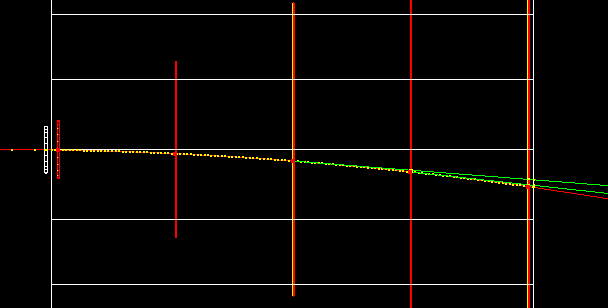
\includegraphics[width=\linewidth]{Immagini/electron.png}
            \end{figure}
        \end{column}
        
    \end{columns}
\end{frame}

\begin{frame}{Exercise 1.1: Energy loss in silicon}
    \begin{columns}[T]
        
        % Left Column: Histogram Placeholder
        \begin{column}{0.5\textwidth}
            \begin{figure}
                \centering
                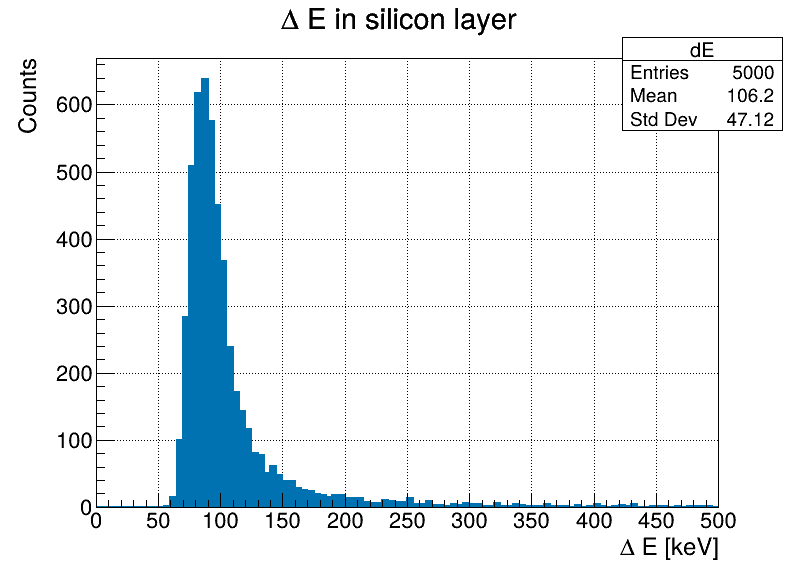
\includegraphics[width=\linewidth]{Immagini/dE.png}
            \end{figure}
        \end{column}
        
        % Right Column: Calculations
        \begin{column}{0.5\textwidth}
            
            \begin{itemize}
                \item Particle: $\mu^-$ at $p = 100\,\mathrm{GeV}/c$ (MIP).
                \item Target: $300\,\mu\mathrm{m}$ Silicon layer.
                \item Calculated expected loss: 
                      \[ \Delta E_{\mathrm{exp}} = \langle \frac{dE}{dx\rho}\rangle\cdot x \rho = 116.2\,\mathrm{keV} \]
            \end{itemize}
            
            
            \begin{itemize}
                \item Extracted mean from \texttt{dE} histogram:
                      \[ \Delta E_{\mathrm{sim}} = 106.2\,\mathrm{keV} \]
            \end{itemize}
            
            
            \begin{itemize}
                \item The relative difference: $\sim9.4\%$
            \end{itemize}
            
        \end{column}
        
    \end{columns}
\end{frame}

\begin{frame}{Exercise 1.2: Multiple scattering in the beam pipe}
    \begin{columns}[T]
        
        % Left Column: Theory & Calculation
        \begin{column}{0.48\textwidth}  
            \small % Riduce leggermente il font per far respirare il testo
            Before reaching the first sensitive layer, a $100\,\mathrm{GeV}/c$ muon experiences multiple scattering primarily inside the $2\,\mathrm{mm}$ Beryllium beam pipe.
            
            \vspace{0.1cm}
            Using the parameterized formula:
            \vspace{-0.1cm}
            $$ \theta_0 = \frac{13.6\,\mathrm{MeV}}{\beta c p} z \sqrt{\frac{x}{X_0}} \left[ 1 + 0.038 \ln \left( \frac{x}{X_0} \right) \right] $$
            \vspace{-0.2cm} % Riduce lo spazio sotto la formula
            
            With $X_0(\text{Be}) \approx 35.3\,\text{cm}$, we obtain:
            $$ \theta_{\mathrm{Be}} \approx 8.22 \times 10^{-6}\,\mathrm{rad} $$ 
            
            \vspace{0.1cm}
            However, the \texttt{theta1st} histogram yields a wider distribution: $\theta_\text{MS} \approx 1.44 \times 10^{-5}\,\mathrm{rad}$.
        \end{column}
        
        % Right Column: Histogram & Explanation
        \begin{column}{0.5\textwidth}
            \vspace{-0.6cm} % Elimina lo spazio bianco sotto la figura

            \begin{figure}
                \centering
                % Immagine ridotta all'85% per fare spazio alla spiegazione
                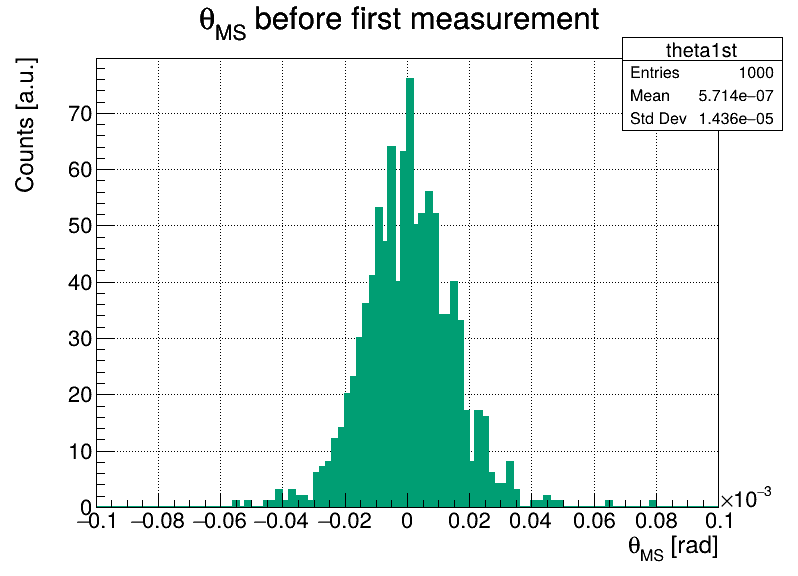
\includegraphics[width=0.85\linewidth, keepaspectratio]{Immagini/theta1st.png}
            \end{figure}
            
            \vspace{-0.5cm} % Elimina lo spazio bianco sotto la figura
            
            \footnotesize % Font più piccolo per il box extra
            \texttt{theta1st} includes both the Be pipe \textbf{and} the $1^{\text{st}}$ tracker layer (Si+C). Summing in quadrature with the layer's theoretical $\theta_\text{MS}$ yields the simulated value:
            \vspace{-0.1cm}
            $$ \theta_{\mathrm{tot}} = \sqrt{\theta_{\mathrm{Be}}^2 + \theta_{\mathrm{layer}}^2} \approx 1.28 \times 10^{-5}\,\mathrm{rad} $$
        \end{column}
        
    \end{columns}
\end{frame}

\begin{frame}{Exercise 1.3: Multiple scattering in a tracker layer}
    \begin{columns}[T]
        
        % Left Column: Theory & Calculation
        \begin{column}{0.48\textwidth}  
            \small % Riduce leggermente il font per far respirare il testo
            A single tracking layer consists of the active $300\,\mu\mathrm{m}$ Silicon sensor backed by a $1\,\mathrm{mm}$ Carbon support ($\rho=2\,\mathrm{g/cm^3}$).
            
            \vspace{0.1cm}
            To apply the parameterized formula to this composite material, we sum the fractional radiation lengths:
            \vspace{-0.1cm}
            $$ \left(\frac{x}{X_0}\right)_{\mathrm{tot}} = \frac{x_{\mathrm{Si}}}{X_{0,\mathrm{Si}}} + \frac{x_{\mathrm{C}}}{X_{0,\mathrm{C}}} $$
            
            Applying the parameterized formula to this composite material yields the theoretical expectation:
            \vspace{-0.1cm}
            $$ \theta_{\mathrm{layer}} =  9.85 \times 10^{-6}\,\mathrm{rad} $$
            \vspace{-0.2cm} 
        
        \end{column}
        
        % Right Column: Histogram & Consistency Check
        \begin{column}{0.5\textwidth}
            \vspace{-0.6cm} 

            \begin{figure}
                \centering
                % Assicurati che il percorso del file sia corretto
                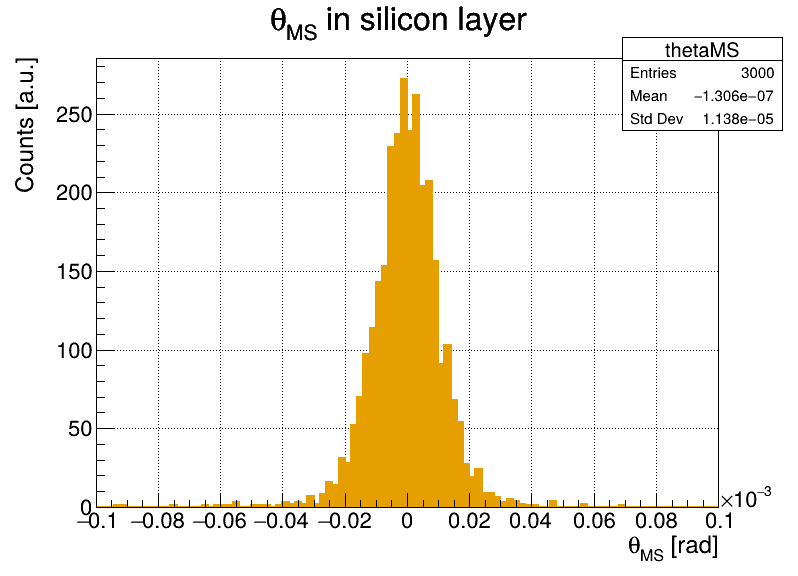
\includegraphics[width=0.85\linewidth, keepaspectratio]{Immagini/thetaMS.png}
            \end{figure}
            
            \vspace{-0.5cm} 
            
            \footnotesize 
            The \texttt{thetaMS} histogram specifically isolates the scattering within this single layer. The simulated value is:
            $$ \theta_{\mathrm{sim}} \approx 1.14 \times 10^{-5}\,\mathrm{rad} $$ 
        \end{column}
        
    \end{columns}
\end{frame}

\begin{frame}{Exercise 1.4: Expected track curvature}
    \begin{columns}[T]
        
        % Left Column: Theory & Calculation
        \begin{column}{0.45\textwidth}  
            A $\mu^-$ with momentum $p = 100\,\mathrm{GeV}/c$ and uniform magnetic field $B = 1\,\mathrm{T}$.
            
            \vspace{0.2cm}
            The track curvature $\kappa = q/R$ can be derived:
            \vspace{-0.1cm}
            $$ p [\text{GeV/c}] = 0.3 \cdot B[T] \cdot R[m]  $$
            $$ \kappa = \frac{-0.3 \cdot B}{p} = -0.003\,\mathrm{m}^{-1}$$
            %\vspace{-0.3cm}
            The extracted \texttt{kappa} histogram exhibits a mean value of $-0.003\,\mathrm{m}^{-1}$.
        \end{column}
        
        % Right Column: Histogram
        \begin{column}{0.55\textwidth}
            \vspace{-0.3cm} 
            \begin{figure}
                \centering
                % Sostituisci "kappa.png" con il nome esatto del tuo file
                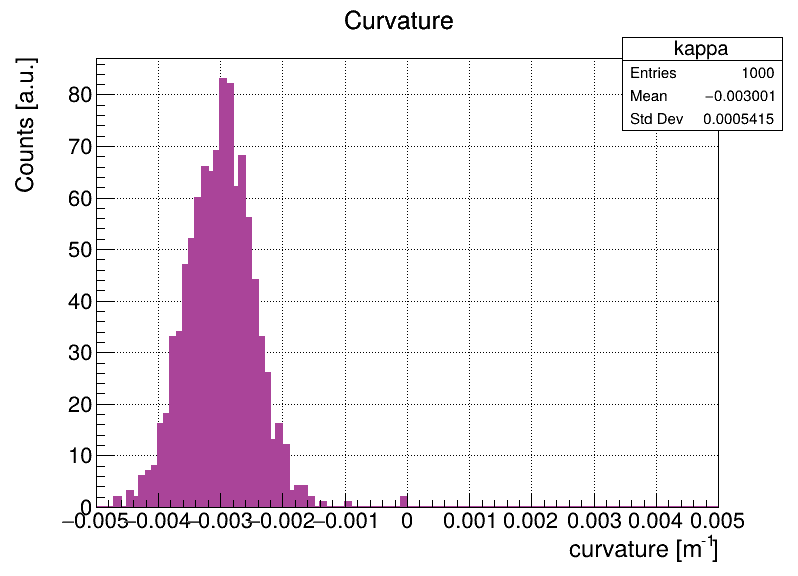
\includegraphics[width=0.98\linewidth, keepaspectratio]{Immagini/kappa.png}
            \end{figure}
            \vspace{-0.6cm}
        \end{column}
        
    \end{columns}
\end{frame}

\begin{frame}{Exercise 1.5: Impact parameter resolution ($d_0$)}
    \begin{columns}[T]
        
        % Right Column: Histogram
        \begin{column}{0.52\textwidth}
            \vspace{-0.3cm} 
            \begin{figure}
                \centering
                % Assicurati che il nome del file immagine sia corretto
                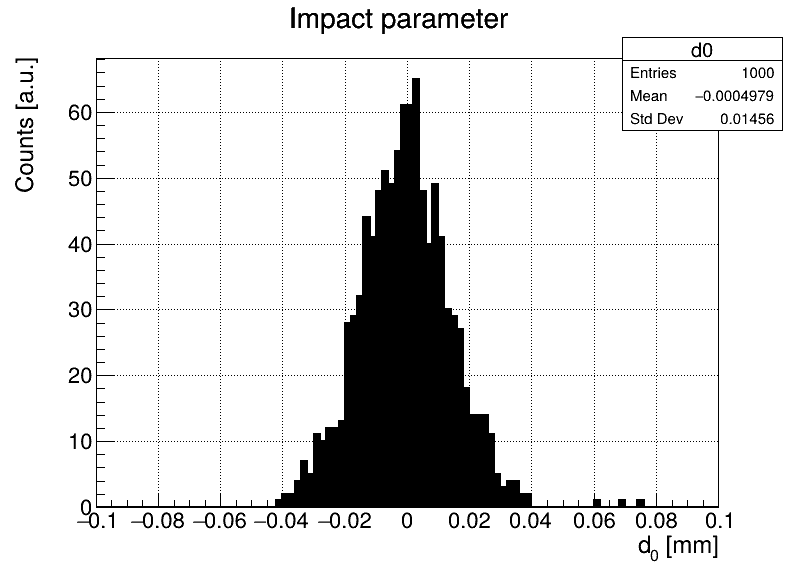
\includegraphics[width=0.98\linewidth, keepaspectratio]{Immagini/d0.png}
            \end{figure}
            \vspace{-0.4cm}
             The \texttt{d0} distribution yields a standard deviation of $\sigma_{\mathrm{sim}} = 14.56\,\mu\mathrm{m}$.
        \end{column}

         % Left Column: Theory & Calculation
        \begin{column}{0.48\textwidth}  
            \small
            The general impact parameter resolution is $\sigma_{d_0} = \sigma_{\mathrm{geom}} \oplus \frac{\sigma_{\mathrm{MS}}}{p\sin^{3/2}\theta}$. For a high-momentum $100\,\mathrm{GeV}/c$ muon, MS becomes negligible, leaving $\sigma_{d_0} \approx \sigma_{\mathrm{geom}}$.
            
            \vspace{0.2cm}
            Applying the 2-plane approximation using the first ($x_1 = 5\,\mathrm{cm}$) and last ($x_2 = 45\,\mathrm{cm}$) layers, the lever arm is $n = x_2/x_1 = 9$.
            
            \vspace{0.2cm}
            Given the intrinsic hit resolution $\sigma_y = 10\,\mu\mathrm{m}$:
            \vspace{-0.1cm}
            $$ \sigma_{d_0} = \sigma_y \frac{\sqrt{1+n^2}}{n-1} = 11.32\,\mu\mathrm{m} $$
        \end{column}
        
    \end{columns}
\end{frame}

\begin{frame}{Exercise 1.6: Curvature resolution}
    \begin{columns}[T]
        
        % Left Column: Mathematical Derivation
        \begin{column}{0.55\textwidth}
            \small
            
            Using the 3-point sagitta method, the curvature $\kappa$ is:
            \vspace{-0.3cm}
            $$ \kappa \approx \frac{8s}{qL^2} $$
            \vspace{-0.5cm}

            The sagitta is measured using three equidistant detector layers ($y_1, y_2, y_3$):
            \vspace{-0.4cm}
            $$ s = y_2 - \frac{y_1 + y_3}{2} $$
            \vspace{-0.5cm}

            Assuming an independent spatial resolution $\sigma_y$ for each layer, the error on the sagitta propagates as:
            \vspace{-0.3cm}
            $$ \sigma_s^2 = \sigma_y^2 + \frac{\sigma_y^2}{4} + \frac{\sigma_y^2}{4} = \frac{3}{2}\sigma_y^2 $$
            \vspace{-0.3cm}
            So, the geometric resolution limit:
            $$ \sigma_\kappa = \frac{8}{L^2}\sqrt{\frac{3}{2}}\sigma_y = \frac{\sqrt{96}}{L^2}\sigma_y $$
        \end{column}
        
        % Right Column: Image and Comparison
        \begin{column}{0.45\textwidth}
            \vspace{-1.3cm}
            \begin{figure}
                \centering
                % Assicurati che il percorso del file sia corretto
                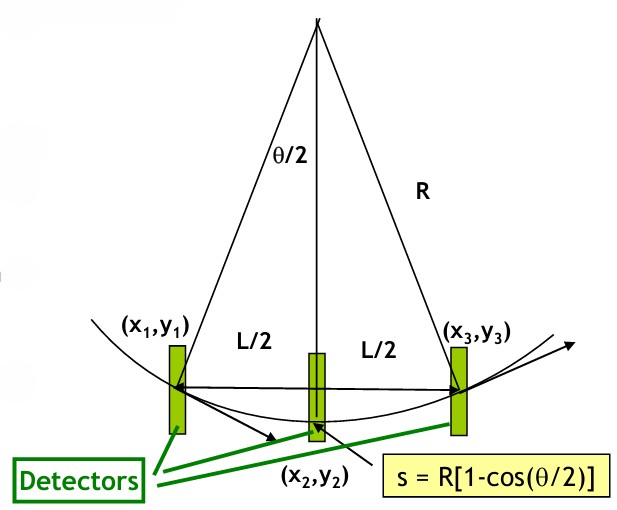
\includegraphics[width=0.6\linewidth, keepaspectratio]{Immagini/saggitta.png}
                \vspace{0.2cm}\\
                \tiny{Source: Prof. Andreazza's Slides}

            \end{figure}
            
            \footnotesize
            Using $L = 40\,\mathrm{cm}$ (distance from $x_1=5$ to $x_3=45\,\mathrm{cm}$) and $\sigma_y = 10\,\mu\mathrm{m}$:
            $$ \sigma_{\kappa,\mathrm{th}} = \frac{\sqrt{96}}{(0.4\,\mathrm{m})^2} \cdot 10^{-5}\,\mathrm{m} = 6.12\times10^{-6}\,\mathrm{m}^{-1} $$
            
            Recalling the simulated \texttt{kappa} resolution:
            $$ \sigma_{\kappa,\mathrm{sim}} = 5.42\times10^{-6}\,\mathrm{m}^{-1} $$
            
        \end{column}
        
    \end{columns}
\end{frame}

\begin{frame}{Exercise 2.1: The parabolic approximation error}
    \begin{columns}[T]
        
        % Left Column: Circle Equation
        \begin{column}{0.48\textwidth}
            \textbf{Exact circular trajectory}
            
            \small
            A track originating at $(0,R)$ with radius $R$ follows a circle:
            $$ z^2 + (y-R)^2 = R^2 $$
            $$ \implies y^2 - 2Ry + z^2 = 0 $$
            
            Solving for the transverse coordinate $y$ (taking the root closest to the origin):
            $$ y_c(z) = R - \sqrt{R^2 - z^2} $$
            $$ y_c(z) = R\left(1 - \sqrt{1 - \left(\frac{z}{R}\right)^2}\right) $$
        \end{column}
        
        % Right Column: Taylor Expansion
        \begin{column}{0.48\textwidth}
            \textbf{Taylor expansion \& error}
            
            \small
            For high-momentum tracks ($z \ll R$), we apply the binomial expansion $\sqrt{1-x} \approx 1 - \frac{x}{2} - \frac{x^2}{8}$:
            $$ y_c(z) \approx R\left[ 1 - \left( 1 - \frac{1}{2}\frac{z^2}{R^2} - \frac{1}{8}\frac{z^4}{R^4} \right) \right] $$
            $$ y_c(z) \approx \frac{z^2}{2R} + \frac{z^4}{8R^3} $$
            
            Tracking algorithms use the parabolic model $y_p(z) = \frac{z^2}{2R}$. The theoretical error is:
            $$ \Delta y = |y_p - y_c| \approx \frac{z^4}{8R^3} $$
        \end{column}
        
    \end{columns}
\end{frame}

\begin{frame}{Exercise 2.2: Magnetic field limit}
    \begin{columns}[T]
        
        % Left Column: Condition and Substitution
        \begin{column}{0.48\textwidth}
            \textbf{Validity condition}
            
            \small
            For a valid approximation, the error at the tracker's edge ($z = L = 0.45\,\mathrm{m}$) must be smaller than the intrinsic hit resolution ($\sigma_y = 10\,\mu\mathrm{m}$).
            \vspace{-0.5cm}
            $$ \Delta y(L) \leq \sigma_y \implies \frac{1}{8} \frac{L^4}{R^3} \leq \sigma_y $$
            
            Substituting  $R = \frac{p}{0.3 B}$:
            $$ \frac{L^4}{8} \left(\frac{0.3 B}{p}\right)^3 \leq \sigma_y $$
            
            $$ \implies B^3 \leq \frac{8 \sigma_y p^3}{(0.3)^3 L^4} $$
        \end{column}
        
        % Right Column: Calculation and Conclusion
        \begin{column}{0.5\textwidth}
            \textbf{Calculation for a low-$p$ muon}
            
            \small
            Evaluating for $p = 0.2\,\mathrm{GeV}/c$:
            $$ B \leq\sqrt[3]{ \frac{8 \cdot (10^{-5}\,\mathrm{m}) \cdot (0.2\,\mathrm{GeV}/c)^3}{0.027 \cdot (0.45\,\mathrm{m})^4}} $$
            $$ \mathbf{B_{\mathrm{max}} \approx 83\,\mathrm{mT}} $$
            
            \small 
            At the nominal field $B = 1\,\mathrm{T}$, for the same $200\,\mathrm{MeV}/c$ track, the bending radius is $R \approx 0.667\,\mathrm{m}$. The approximation error becomes $\Delta y \approx 1.73\,\mathrm{cm}$, completely surpassing the $10\,\mu\mathrm{m}$ detector resolution.
        \end{column}
        
    \end{columns}
\end{frame}

\begin{frame}{Exercise 2.3: Mean energy loss vs momentum}
    \begin{columns}[T]
        \begin{column}{0.4\textwidth}
            \small
            The simulated mean energy loss perfectly reproduces the theoretical Bethe-Bloch behavior for muons ($200\,\text{MeV}/c-200\,\text{GeV}/c$).
            
            \begin{itemize}
                \item \textbf{Low momentum:} The sharp initial drop scales as $1/\beta^2$.
                \item \textbf{MIP regime:} The minimum ionizing region occurs around $p \approx 1\,\mathrm{GeV}/c$.
                \item \textbf{Relativistic rise:} A logarithmic relativistic increase is visible at higher momenta.
            \end{itemize}
            
        \end{column}
        
        \begin{column}{0.6\textwidth}
            \vspace{-0.3cm}
            \begin{figure}
                \centering
                % Inserisci il nome corretto del file
                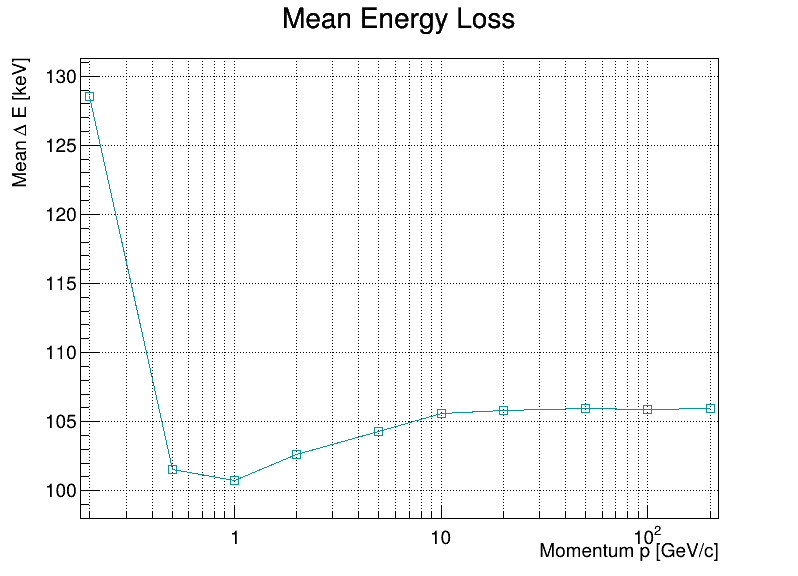
\includegraphics[width=0.98\linewidth, keepaspectratio]{Immagini/dE_mean_vs_p.png}
            \end{figure}
            \footnotesize \textit{Note:} The y-axis does not start at zero to clearly highlight these fine-scale features.
        \end{column}
    \end{columns}
\end{frame}

\begin{frame}{Exercise 2.3: Multiple scattering angle}
    \begin{columns}[T]
        \begin{column}{0.45\textwidth}
            \small
            The multiple Coulomb scattering angle is inversely proportional to momentum:
            $$ \theta_0 \propto \frac{1}{\beta c p} \sqrt{\frac{x}{X_0}} $$
            
            For relativistic particles ($\beta \to 1$), taking the logarithm yields:
            $$ \log(\theta_0) = -\log(p) + C $$
            
            As expected, the simulation perfectly follows a straight line with a slope of $-1$ on the log-log plot.
        \end{column}
        
        \begin{column}{0.55\textwidth}
            \vspace{-0.3cm}
            \begin{figure}
                \centering
                % Inserisci il nome corretto del file
                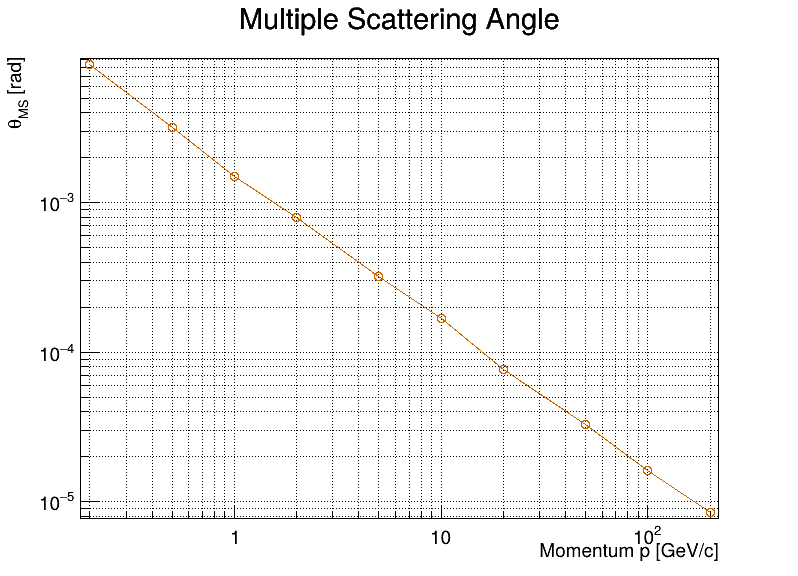
\includegraphics[width=0.98\linewidth, keepaspectratio]{Immagini/thetaMS_vs_p.png}
            \end{figure}
        \end{column}
    \end{columns}
\end{frame}

\begin{frame}{Exercise 2.3: Impact parameter \& direction resolutions}

    % --- Parte superiore: Testo a tutta larghezza ---
    Both $\sigma_{d_0}$ and $\sigma_{\phi_0}$ exhibit the same dual behavior, governed by: $\sigma = A_{\mathrm{geom}} \oplus \frac{B_{\mathrm{MS}}}{p}$    
    \vspace{-0.1cm} % Riduce un po' lo spazio sotto la formula
    \begin{itemize}
        \item \textbf{MS dominated ($p < 10\,\mathrm{GeV}/c$):} The resolution degrades rapidly as $1/p$, completely dominating the error.
        \item \textbf{Intrinsic limit ($p > 10\,\mathrm{GeV}/c$):} The MS term vanishes, and the resolution asymptotes to the purely geometric detector limit ($\propto \sigma_y$).
    \end{itemize}
    
    \vspace{-0.4cm}
    
    % --- Parte inferiore: Due grafici affiancati ---
    \begin{columns}[T]
        \begin{column}{0.5\textwidth}
            \begin{figure}
                \centering
                % Aggiunto parametro height per evitare che sforino in basso
                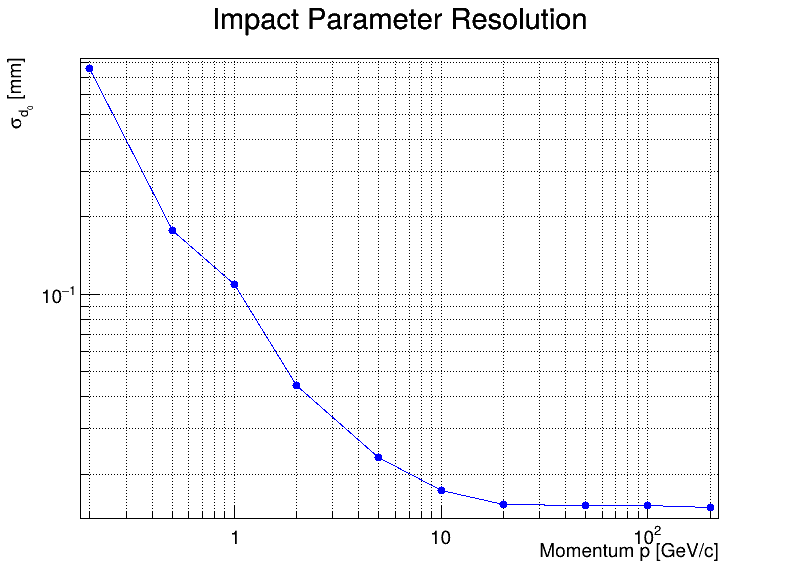
\includegraphics[width=0.8\linewidth, keepaspectratio]{Immagini/sigma_d0_vs_p.png}
            \end{figure}
        \end{column}
        
        \begin{column}{0.5\textwidth}
            \begin{figure}
                \centering
                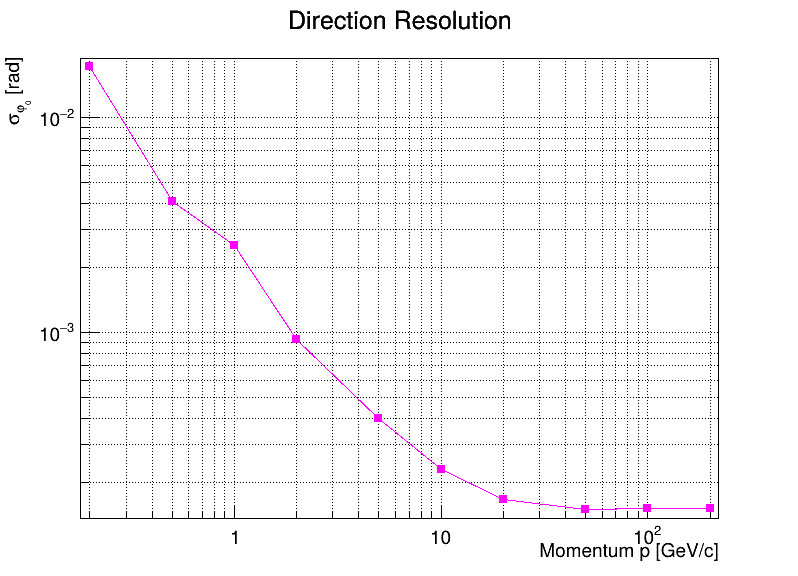
\includegraphics[width=0.8\linewidth, keepaspectratio]{Immagini/sigma_phi0_vs_p.png}
            \end{figure}
        \end{column}
    \end{columns}

\end{frame}

\begin{frame}{Exercise 2.3: Curvature resolution ($\sigma_\kappa$)}
    \begin{columns}[T]
        \begin{column}{0.4\textwidth}
            \small
            The curvature resolution also follows the $\sigma = A_{\mathrm{geom}} \oplus \frac{B_{\mathrm{MS}}}{p}$ rule.
            
            To understand the momentum resolution, we link it to $\kappa$. From $p = 0.3 B / \kappa$, we propagate the error by differentiating:
            $$ \left| \frac{dp}{d\kappa} \right| = \frac{0.3 B}{\kappa^2} = \frac{p}{\kappa} $$
            
            Therefore, the absolute error on momentum is $\sigma_p = \frac{p}{\kappa}\sigma_\kappa$, which leads to:
            $$ \frac{\sigma_p}{p} = \frac{\sigma_\kappa}{\kappa} $$
        \end{column}
        
        \begin{column}{0.6\textwidth}
            \vspace{-0.3cm}
            \begin{figure}
                \centering
                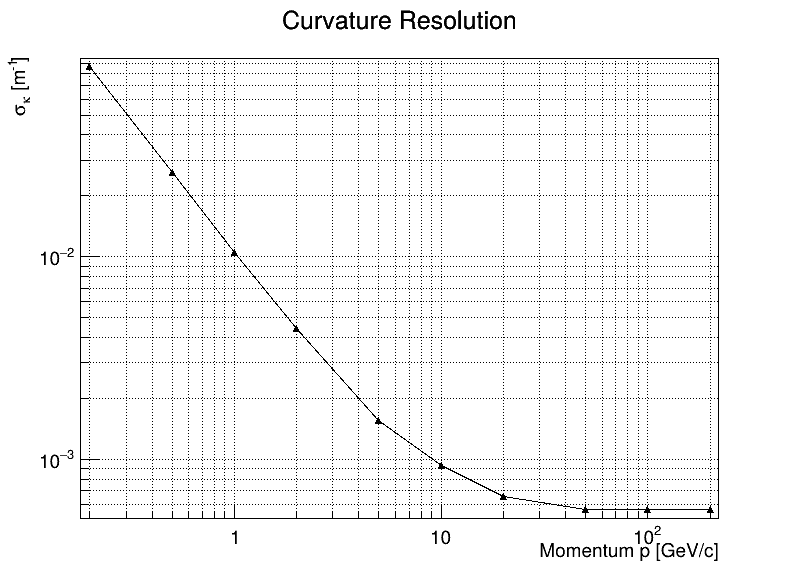
\includegraphics[width=0.98\linewidth, keepaspectratio]{Immagini/sigma_kappa_vs_p.png}
            \end{figure}
        \end{column}
    \end{columns}
\end{frame}

\begin{frame}{Exercise 2.3: Relative momentum resolution ($\sigma_p / p$)}
    \begin{columns}[T]
        \begin{column}{0.48\textwidth}
            
            \footnotesize
            Substituting $\kappa \propto 1/p$, the behavior flips:
            $$ \frac{\sigma_p}{p} = \sqrt{\left(\underbrace{A \cdot p}_{\mathrm{Geom}}\right)^2 + \underbrace{B^2}_{\mathrm{MS}}} $$
            
            \vspace{0.3cm}
            \textbf{Parabolic failure at low $p$}
            
            \footnotesize
            At $p=0.2\,\mathrm{GeV}/c$, $R = 66.7\,\mathrm{cm}$. The track is no longer a small arc but sweeps a huge angle ($\theta \approx 38^\circ$) inside the tracker, completely breaking the parabolic approximation $\Delta y = \frac{z^4}{8R^3}$.
        \end{column}
        
        \begin{column}{0.52\textwidth}
            \vspace{-0.2cm}
            \begin{figure}
                \centering
                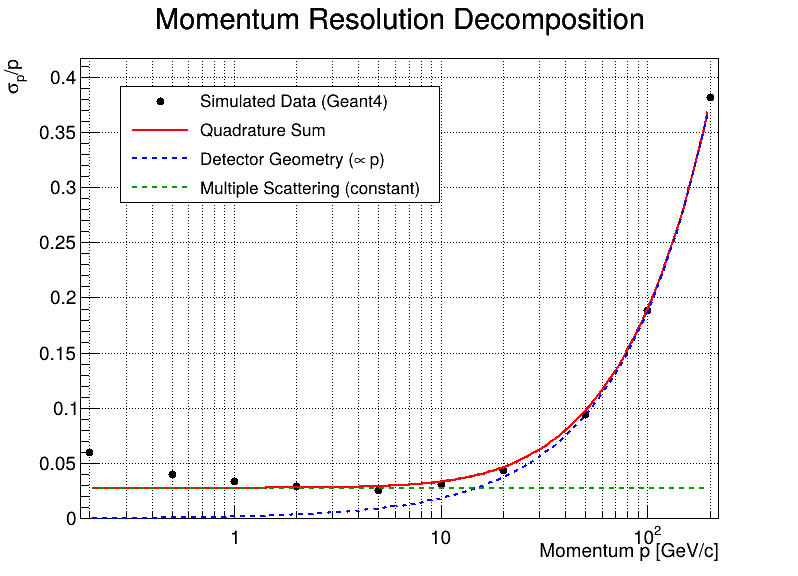
\includegraphics[width=0.98\linewidth, keepaspectratio]{Immagini/sigma_p_decomposition.png}
            \end{figure}
        \end{column}
    \end{columns}
\end{frame}



% --- INIZIO SLIDES ESERCIZIO 3 ---

% Frame 1: 500 MeV - Curvature and Radius
%\begin{frame}{Exercise 3.1: Particle ID at 500 MeV/c ($\kappa$ \& $R$)}
%    \small
%    \begin{itemize}
%        \item \textbf{Bremsstrahlung:} The electron loses momentum ($p$) radiatively. Since $\kappa \propto 1/p$, its trajectory curls irregularly.
%        \item \textbf{Asymmetric Tail:} This produces a prominent tail towards larger negative $\kappa$. Muons and pions do not radiate, keeping constant $\kappa$.
%    \end{itemize}
%    \vspace{0.1cm}
%    \begin{columns}
%        \begin{column}{0.5\textwidth}
%            \centering
%            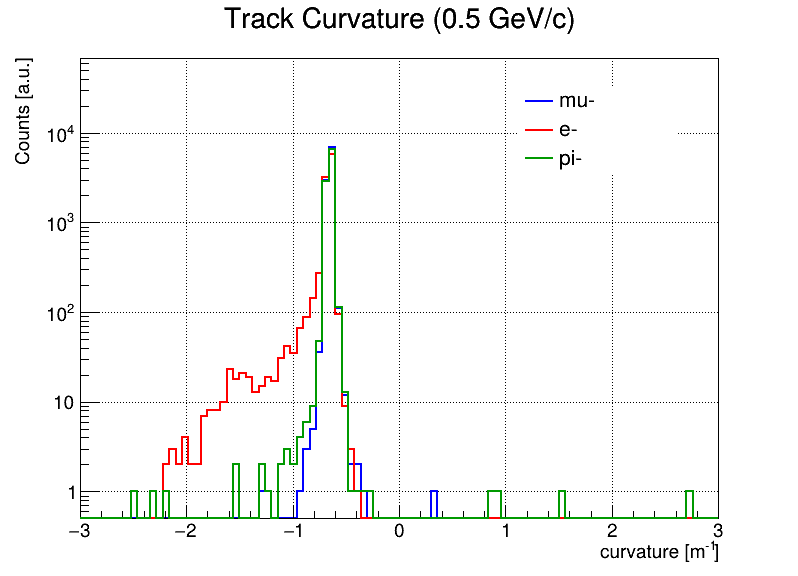
\includegraphics[width=0.8\linewidth]{Immagini/confronto_kappa_0.5GeV.png}
%        \end{column}
%        \begin{column}{0.5\textwidth}
%            \centering
%            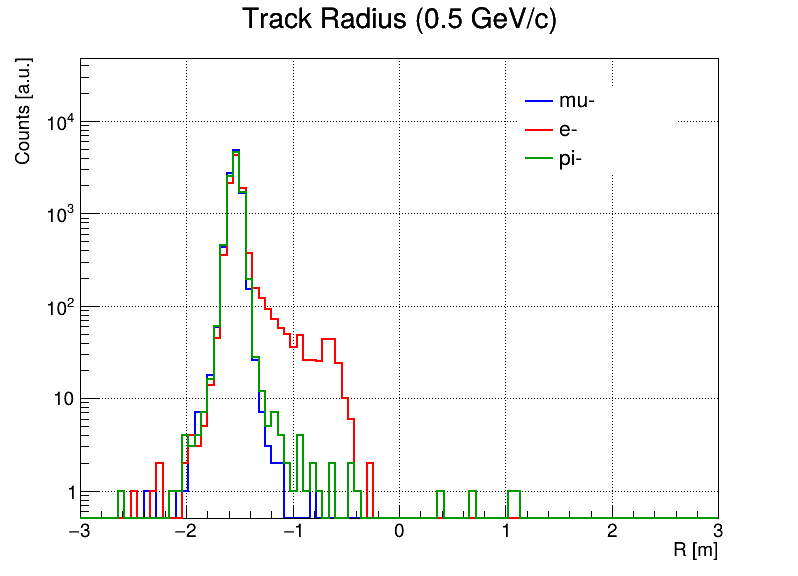
\includegraphics[width=0.8\linewidth]{Immagini/confronto_R_0.5GeV.png}
%        \end{column}
%    \end{columns}
%\end{frame}

% Frame 2: 500 MeV - Impact Parameter and Azimuthal Angle
%\begin{frame}{Exercise 3.1: Particle ID at 500 MeV/c ($d_0$ \& $\phi_0$)}
%    \small
%    \begin{itemize}
%    \item \textbf{Tracking Assumption:} Algorithms assume smooth ionization paths (like $\mu/\pi$). At 500 MeV, $e^-$ Bremsstrahlung drops instead.
%\end{itemize}
%    \vspace{0.1cm}
%    \begin{columns}
%        \begin{column}{0.5\textwidth}
%            \centering
%            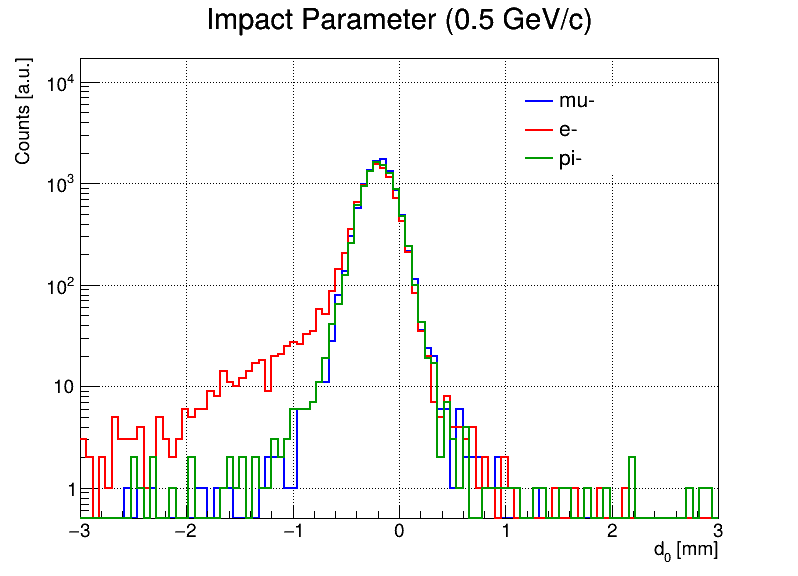
\includegraphics[width=0.8\linewidth]{Immagini/confronto_d0_0.5GeV.png}
%        \end{column}
%        \begin{column}{0.5\textwidth}
%            \centering
%            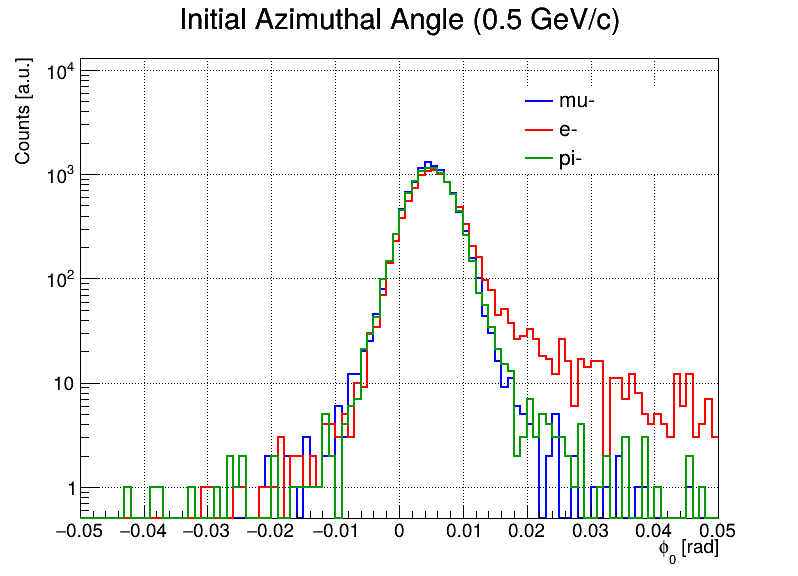
\includegraphics[width=0.8\linewidth]{Immagini/confronto_phi0_0.5GeV.png}
%        \end{column}
%    \end{columns}
%\end{frame}

% Frame 3: 500 MeV - Number of Steps
%\begin{frame}{Exercise 3.1: Particle ID at 500 MeV/c (Number of Steps)}
%    \small
%    \begin{itemize}
%        \item \textbf{Geant4 Steps:} Charged particles typically cross a thin silicon layer in a single simulation step.
%        \item \textbf{Radiative Signature:} Multiple steps indicate significant energy losses. The long tail for $e^-$ is a direct signature of Bremsstrahlung.
%    \end{itemize}
%    \begin{figure}
%        \centering
%        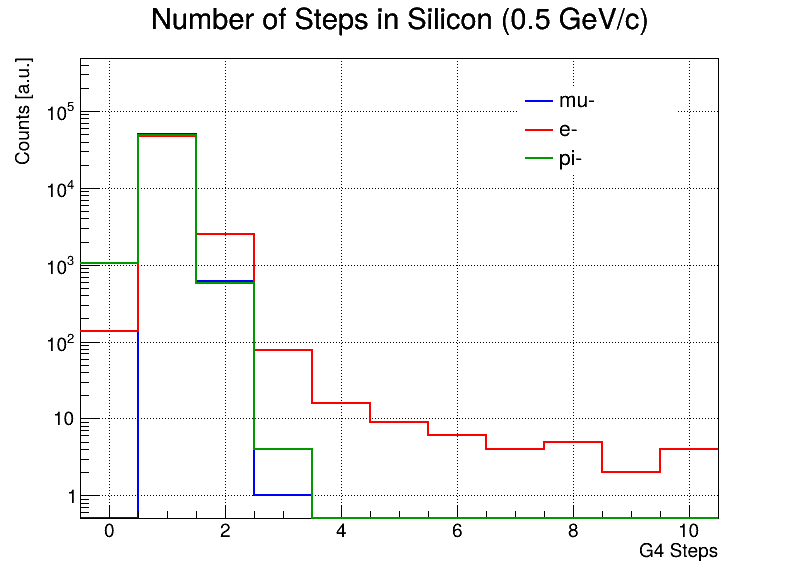
\includegraphics[width=0.45\linewidth]{Immagini/confronto_nstep_0.5GeV.png}
%    \end{figure}
%\end{frame}










% Frame 1: 500 MeV - Curvature and Radius
\begin{frame}{Exercise 3.1: 500 MeV/c ($\kappa$ \& $R$)}
    \small
    \begin{itemize}
        \item While $\mu^-$ and $\pi^-$ lose energy steadily via ionization, $e^-$ can do Bremsstrahlung at any point in the tracker.
        \item A sudden drop in $p$ causes the trajectory to curl tighter ($\kappa \propto 1/p$). The global fit averages this anomaly, creating prominent asymmetric tails.
    \end{itemize}
    \vspace{0.1cm}
    \begin{columns}
        \begin{column}{0.5\textwidth}
            \centering
            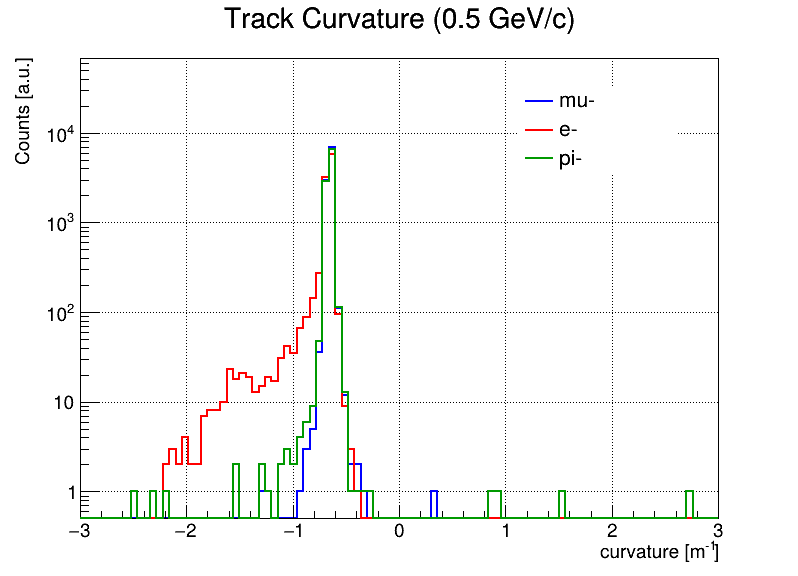
\includegraphics[width=0.8\linewidth]{Immagini/confronto_kappa_0.5GeV.png}
        \end{column}
        \begin{column}{0.5\textwidth}
            \centering
            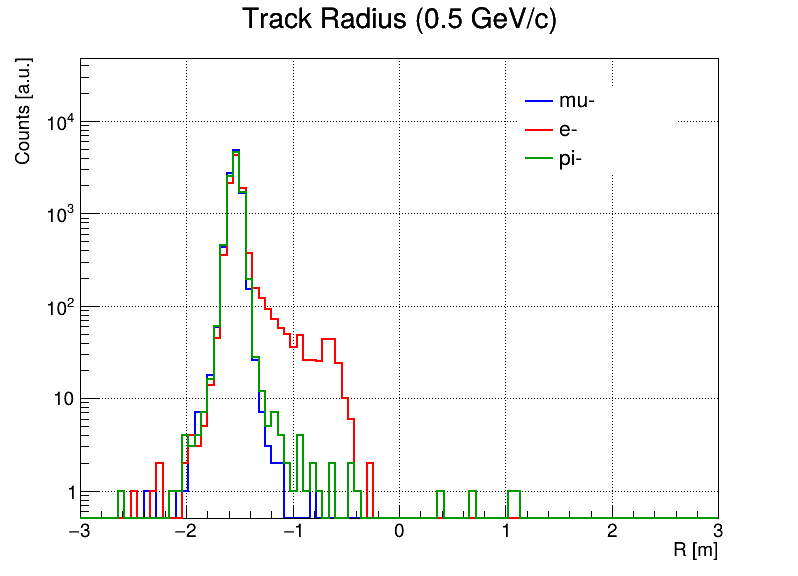
\includegraphics[width=0.8\linewidth]{Immagini/confronto_R_0.5GeV.png}
        \end{column}
    \end{columns}
\end{frame}

% Frame 2: 500 MeV - Impact Parameter and Azimuthal Angle
\begin{frame}{Exercise 3.1: 500 MeV/c ($d_0$ \& $\phi_0$)}
    \small
    The origin is reconstructed by assuming continuous energy loss. This produces the non-perfectly symmetric distributions observed for $d_0$ and $\phi_0$.
    \vspace{0.1cm}
    \begin{columns}
        \begin{column}{0.5\textwidth}
            \centering
            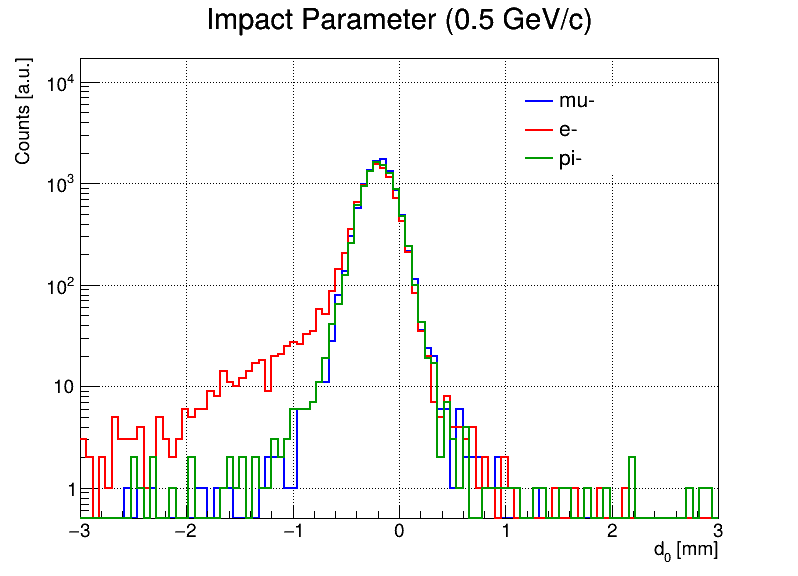
\includegraphics[width=0.85\linewidth]{Immagini/confronto_d0_0.5GeV.png}
        \end{column}
        \begin{column}{0.5\textwidth}
            \centering
            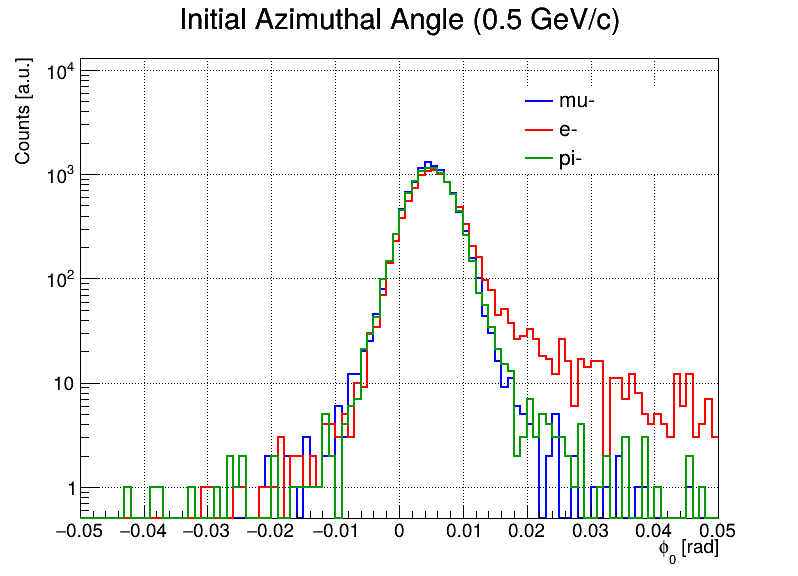
\includegraphics[width=0.85\linewidth]{Immagini/confronto_phi0_0.5GeV.png}
        \end{column}
    \end{columns}
\end{frame}

\begin{frame}{Exercise 3.1: 500 MeV/c (Number of steps)}
    \small
    \begin{columns}
        \begin{column}{0.55\textwidth}
            \begin{itemize}
                \item Geant4 typically simulates a MIP crossing a thin silicon layer in a single step (ionization).
                \item To generate a secondary Bremsstrahlung photon, Geant4 must interrupt and split the step. The $e^-$ tail is the direct microscopic proof of these discrete events.
                \item The material is minimal ($\sim 4.5\% \, X_0$), making hard Bremsstrahlung statistically rare. The logarithmic scale is crucial to reveal this small fraction of non-ideal events against the bulk behavior.
            \end{itemize}
        \end{column}
        \begin{column}{0.45\textwidth}
            \centering
            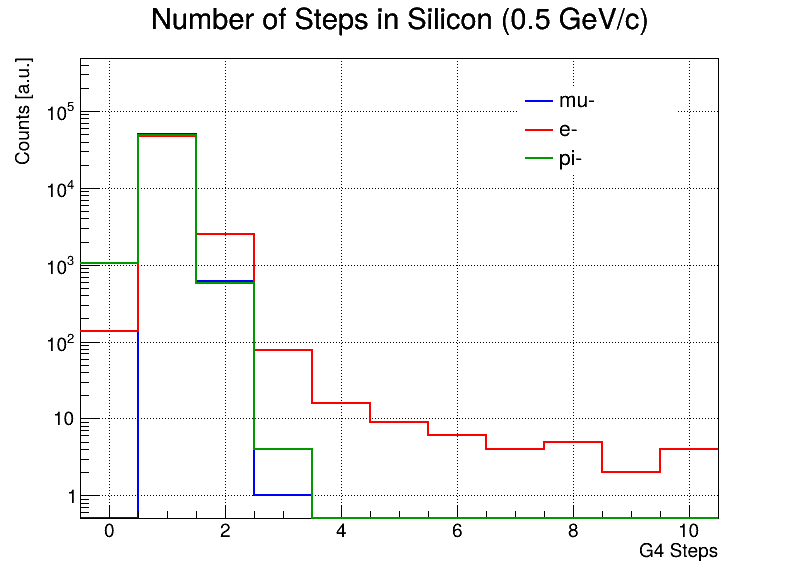
\includegraphics[width=\linewidth]{Immagini/confronto_nstep_0.5GeV.png}
        \end{column}
    \end{columns}
\end{frame}











% Frame 4: 100 GeV - Impact Parameter and Azimuthal Angle
%\begin{frame}{Exercise 3.1: Kinematic at 100 GeV/c ($d_0$ \& $\phi_0$)}
%    \small
%    \begin{itemize}
%        \item \textbf{MS Suppression:} Scaling as $1/p$, multiple scattering becomes negligible compared to the intrinsic spatial resolution of silicon.
%        \item \textbf{Rigid Tracks:} Straight trajectories lead to highly accurate backward extrapolation, collapsing the $d_0$ and $\phi_0$ distributions together.
%    \end{itemize}
%    \vspace{0.1cm}
%    \begin{columns}
%        \begin{column}{0.5\textwidth}
%            \centering
%            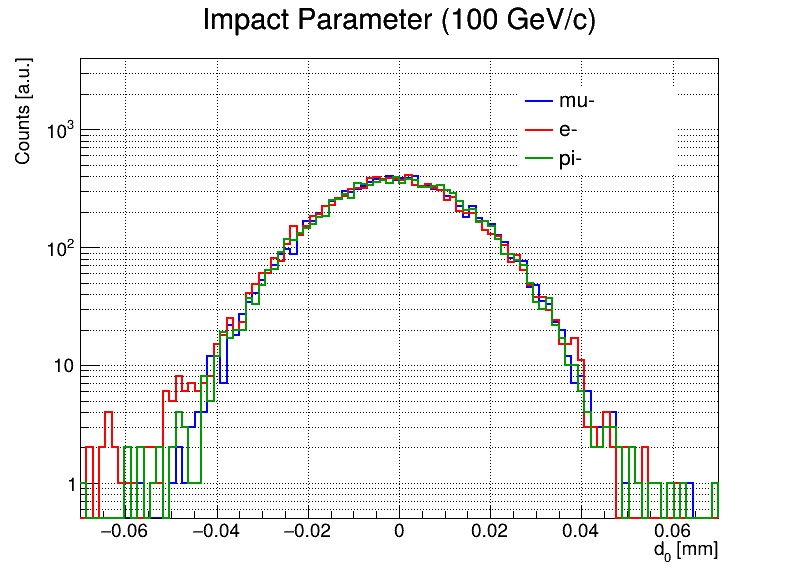
\includegraphics[width=0.8\linewidth]{Immagini/confronto_d0_100GeV.png}
%        \end{column}
%        \begin{column}{0.5\textwidth}
%            \centering
%            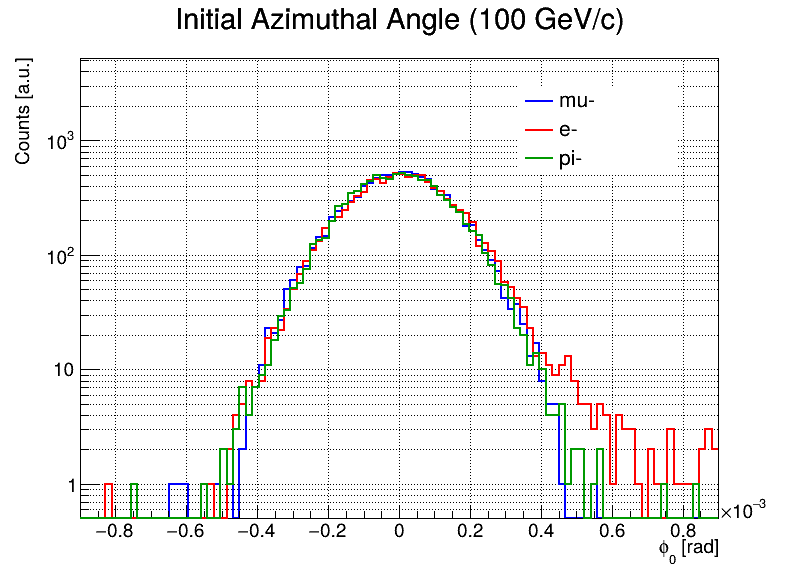
\includegraphics[width=0.8\linewidth]{Immagini/confronto_phi0_100GeV.png}
%        \end{column}
%    \end{columns}
%\end{frame}

% Frame 5: 100 GeV - Curvature, Radius & Pion Behavior
%\begin{frame}{Exercise 3.1: Kinematic at 100 GeV/c ($\kappa$ \& $R$)}
%    \small
%    \begin{itemize}
%        \item \textbf{Residual Radiation:} The $e^-$ still radiates at 100 GeV/c. Momentum loss preserves the characteristic asymmetric curvature tail.
%        \item \textbf{Silent Pions:} The SiTracker is too thin ($300~\mu\text{m} \ll \lambda_{int}$) to induce hadronic showers. Pions behave exactly like muons. %   \end{itemize}
%   \vspace{0.1cm}
%   \begin{columns}
%        \begin{column}{0.5\textwidth}
%            \centering
%            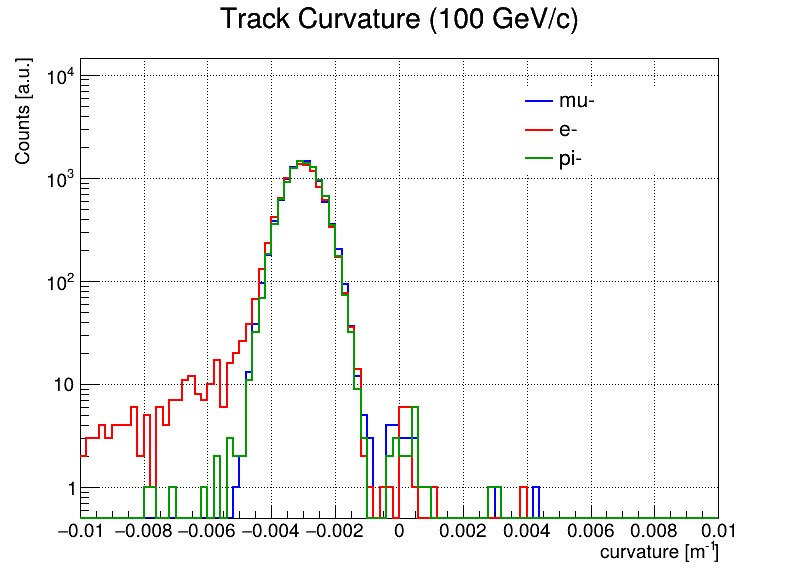
\includegraphics[width=0.8\linewidth]{Immagini/confronto_kappa_100GeV.png}
%        \end{column}
%        \begin{column}{0.5\textwidth}
%            \centering
%            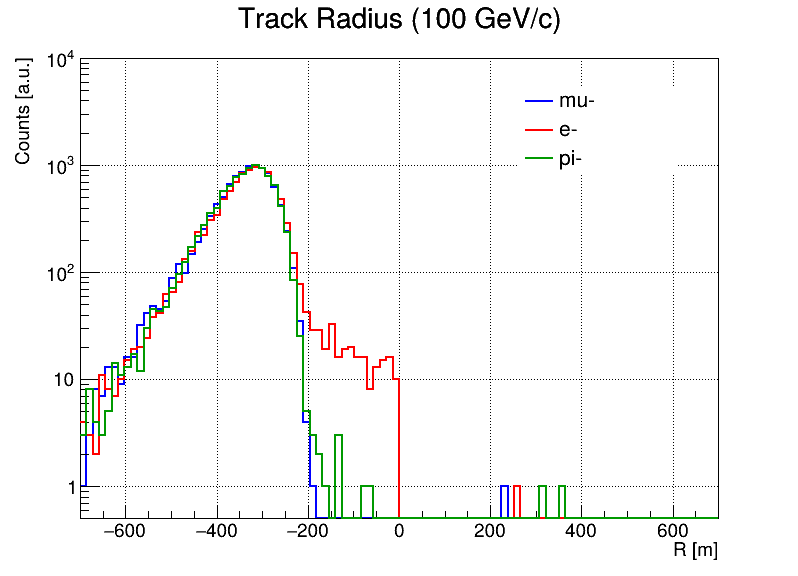
\includegraphics[width=0.8\linewidth]{Immagini/confronto_R_100GeV.png}
%        \end{column}
%    \end{columns}
%\end{frame}










% Frame 4: 100 GeV - Curvature, Radius & Pion Behavior
\begin{frame}{Exercise 3.1: 100 GeV/c ($\kappa$ \& $R$)}
    \small
    \begin{itemize}
        \item The $e^-$ still radiates at 100 GeV/c. The continuous loss of momentum preserves the characteristic asymmetric tail.
        \item The SiTracker is too thin ($300~\mu\text{m} \ll \lambda_{int}$) to induce hadronic showers. In this case (as well as for $500\,\text{MeV}$ particles), pions behave exactly like muons.
    \end{itemize}
    \vspace{0.1cm}
    \begin{columns}
        \begin{column}{0.5\textwidth}
            \centering
            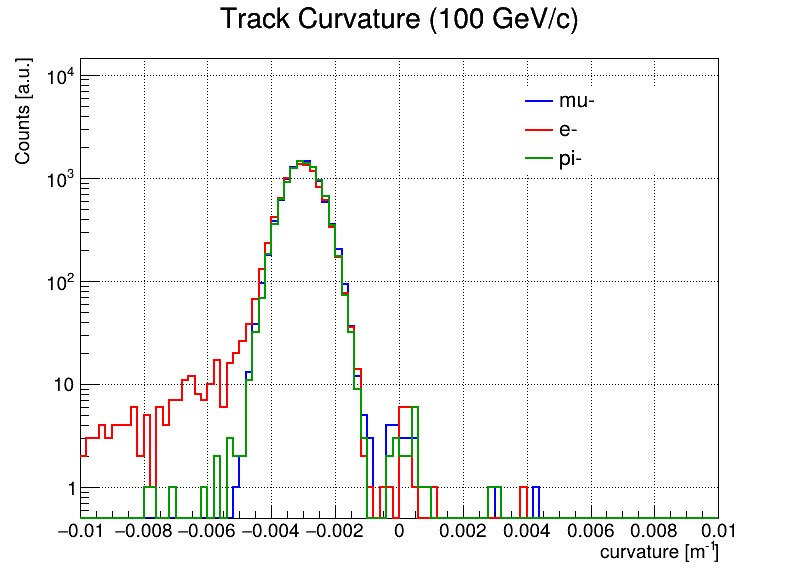
\includegraphics[width=0.8\linewidth]{Immagini/confronto_kappa_100GeV.png}
        \end{column}
        \begin{column}{0.5\textwidth}
            \centering
            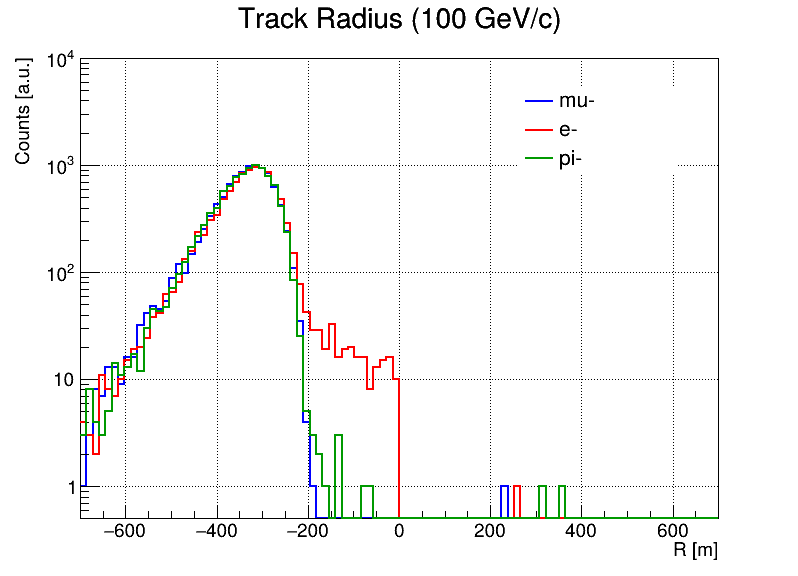
\includegraphics[width=0.8\linewidth]{Immagini/confronto_R_100GeV.png}
        \end{column}
    \end{columns}
\end{frame}

% Frame 5: 100 GeV - Impact Parameter and Azimuthal Angle
\begin{frame}{Exercise 3.1: 100 GeV/c ($d_0$ \& $\phi_0$)}
        Despite the radiation shown previously, the tracks are now so rigid that the impact parameter and azimuthal angle are completely unaffected.
    \vspace{0.1cm}
    \begin{columns}
        \begin{column}{0.5\textwidth}
            \centering
            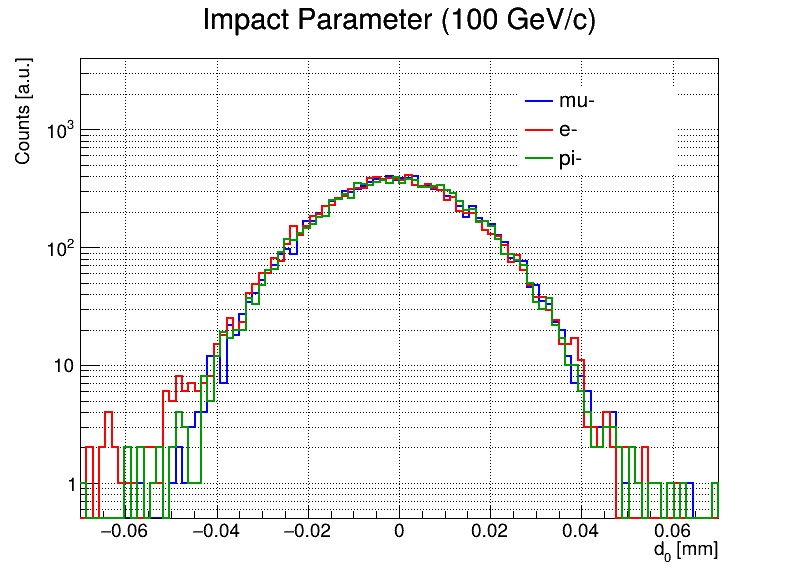
\includegraphics[width=0.9\linewidth]{Immagini/confronto_d0_100GeV.png}
        \end{column}
        \begin{column}{0.5\textwidth}
            \centering
            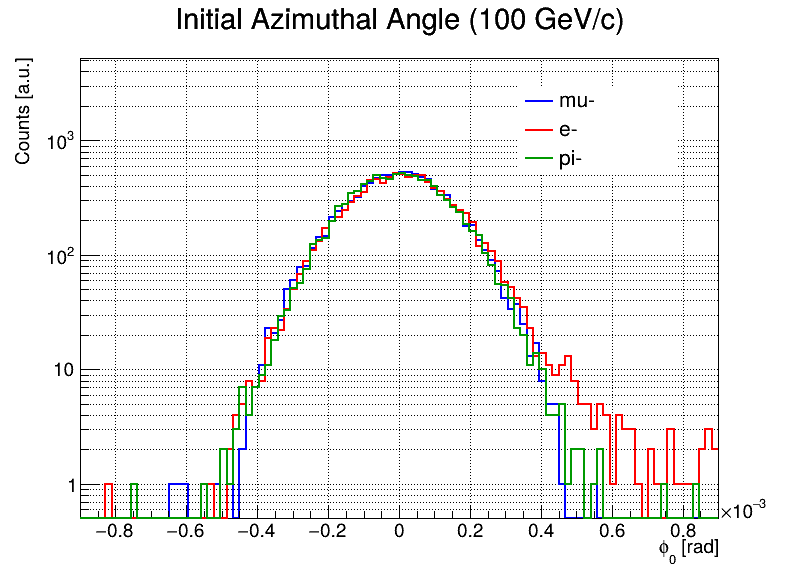
\includegraphics[width=0.9\linewidth]{Immagini/confronto_phi0_100GeV.png}
        \end{column}
    \end{columns}
\end{frame}










% Frame 6: Conclusions
%\begin{frame}{Exercise 3.1: Conclusions on Detector Architecture}
%    \small
%    \begin{itemize}
%        \item \textbf{Inner Placement:} The 100 GeV/c data explains why trackers in ATLAS/CMS are placed closest to the interaction point.
%        \item \textbf{Minimal Perturbation:} The goal is to measure momentum without altering the particle's trajectory.
%        \item \textbf{Material Budget:} Excess material would degrade energy prematurely, spoiling downstream measurements in the calorimeters.
%    \end{itemize}
%\end{frame}

% --- FINE SLIDES ESERCIZIO 3 ---



\begin{frame}{Exercise 3.2: Local parameters resolution ($d_0$ \& $\phi_0$)}
    \begin{itemize}
        \item \textbf{Impact parameter ($d_0$):} Resolution improves monotonically, driven by the increased statistical sampling near the interaction point.
        \item \textbf{Azimuthal angle ($\phi_0$):} Exhibits a similar trend, being primarily sensitive to the first few layers before significant material effects accumulate.
    \end{itemize}
    
    
    \begin{columns}
        \begin{column}{0.5\textwidth}
            \centering
            % Assicurati che il path dell'immagine sia corretto
            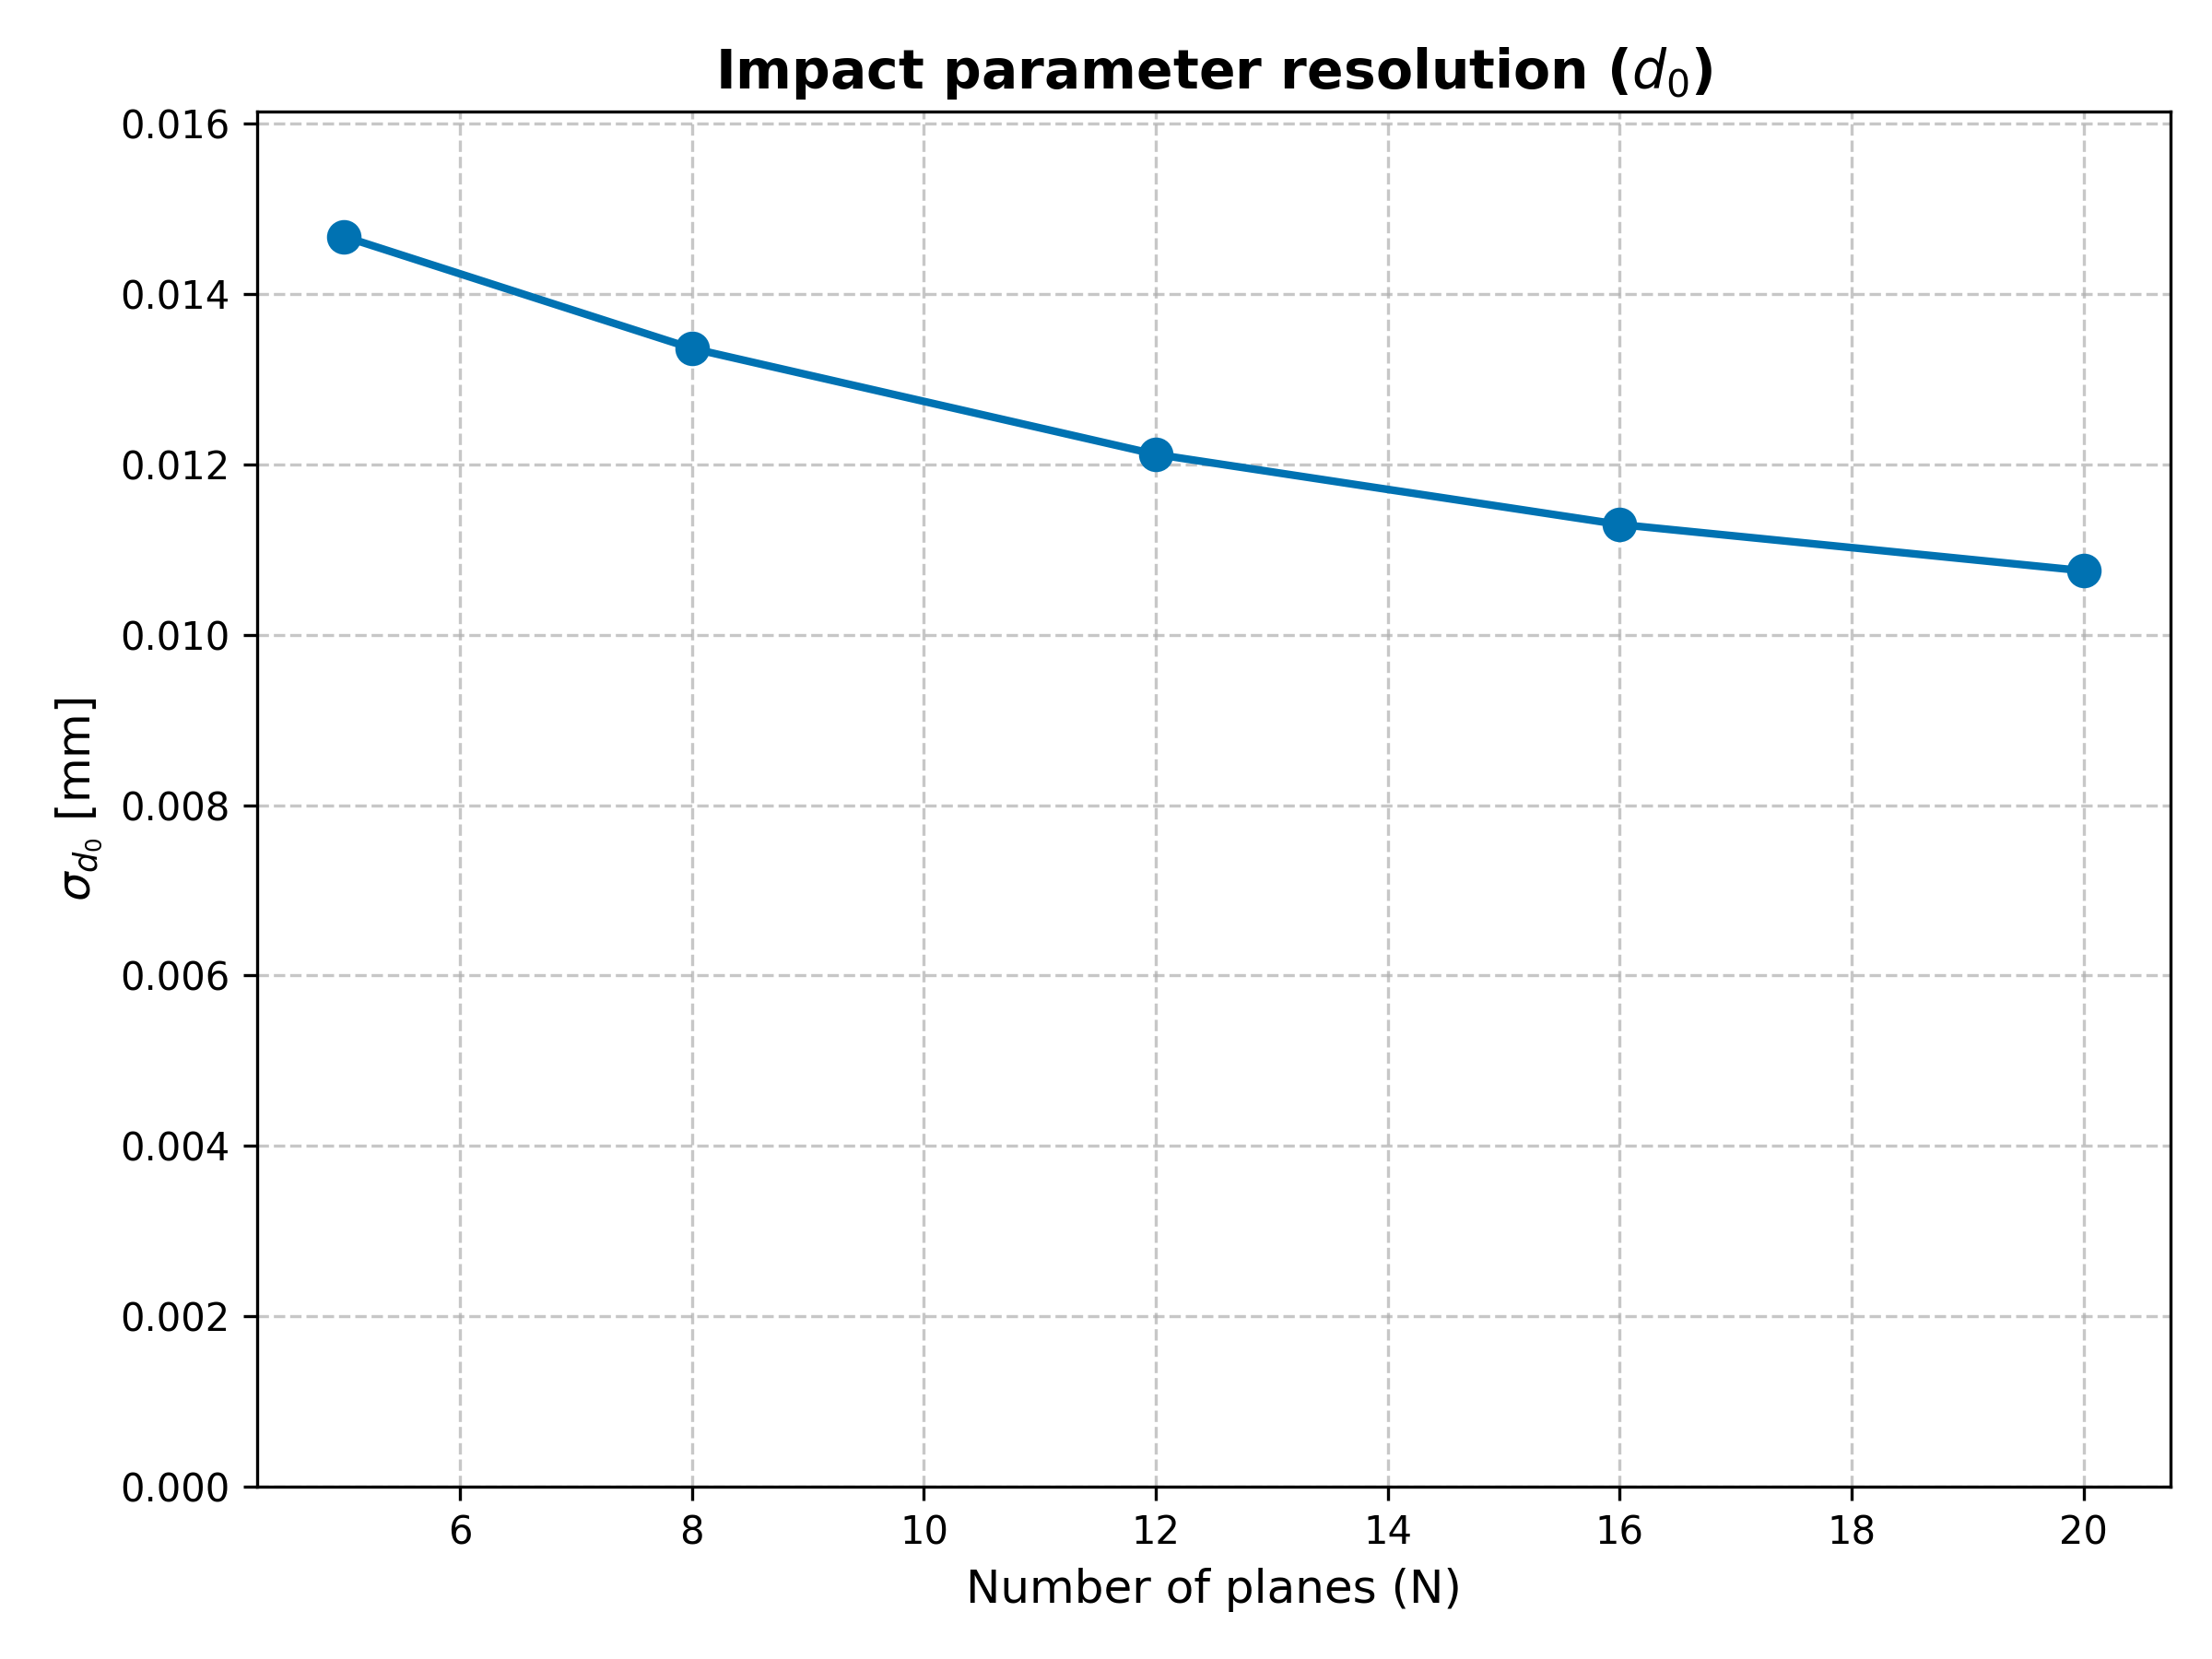
\includegraphics[width=0.85\textwidth]{Immagini/trend_d0.png}
        \end{column}
        \begin{column}{0.5\textwidth}
            \centering
            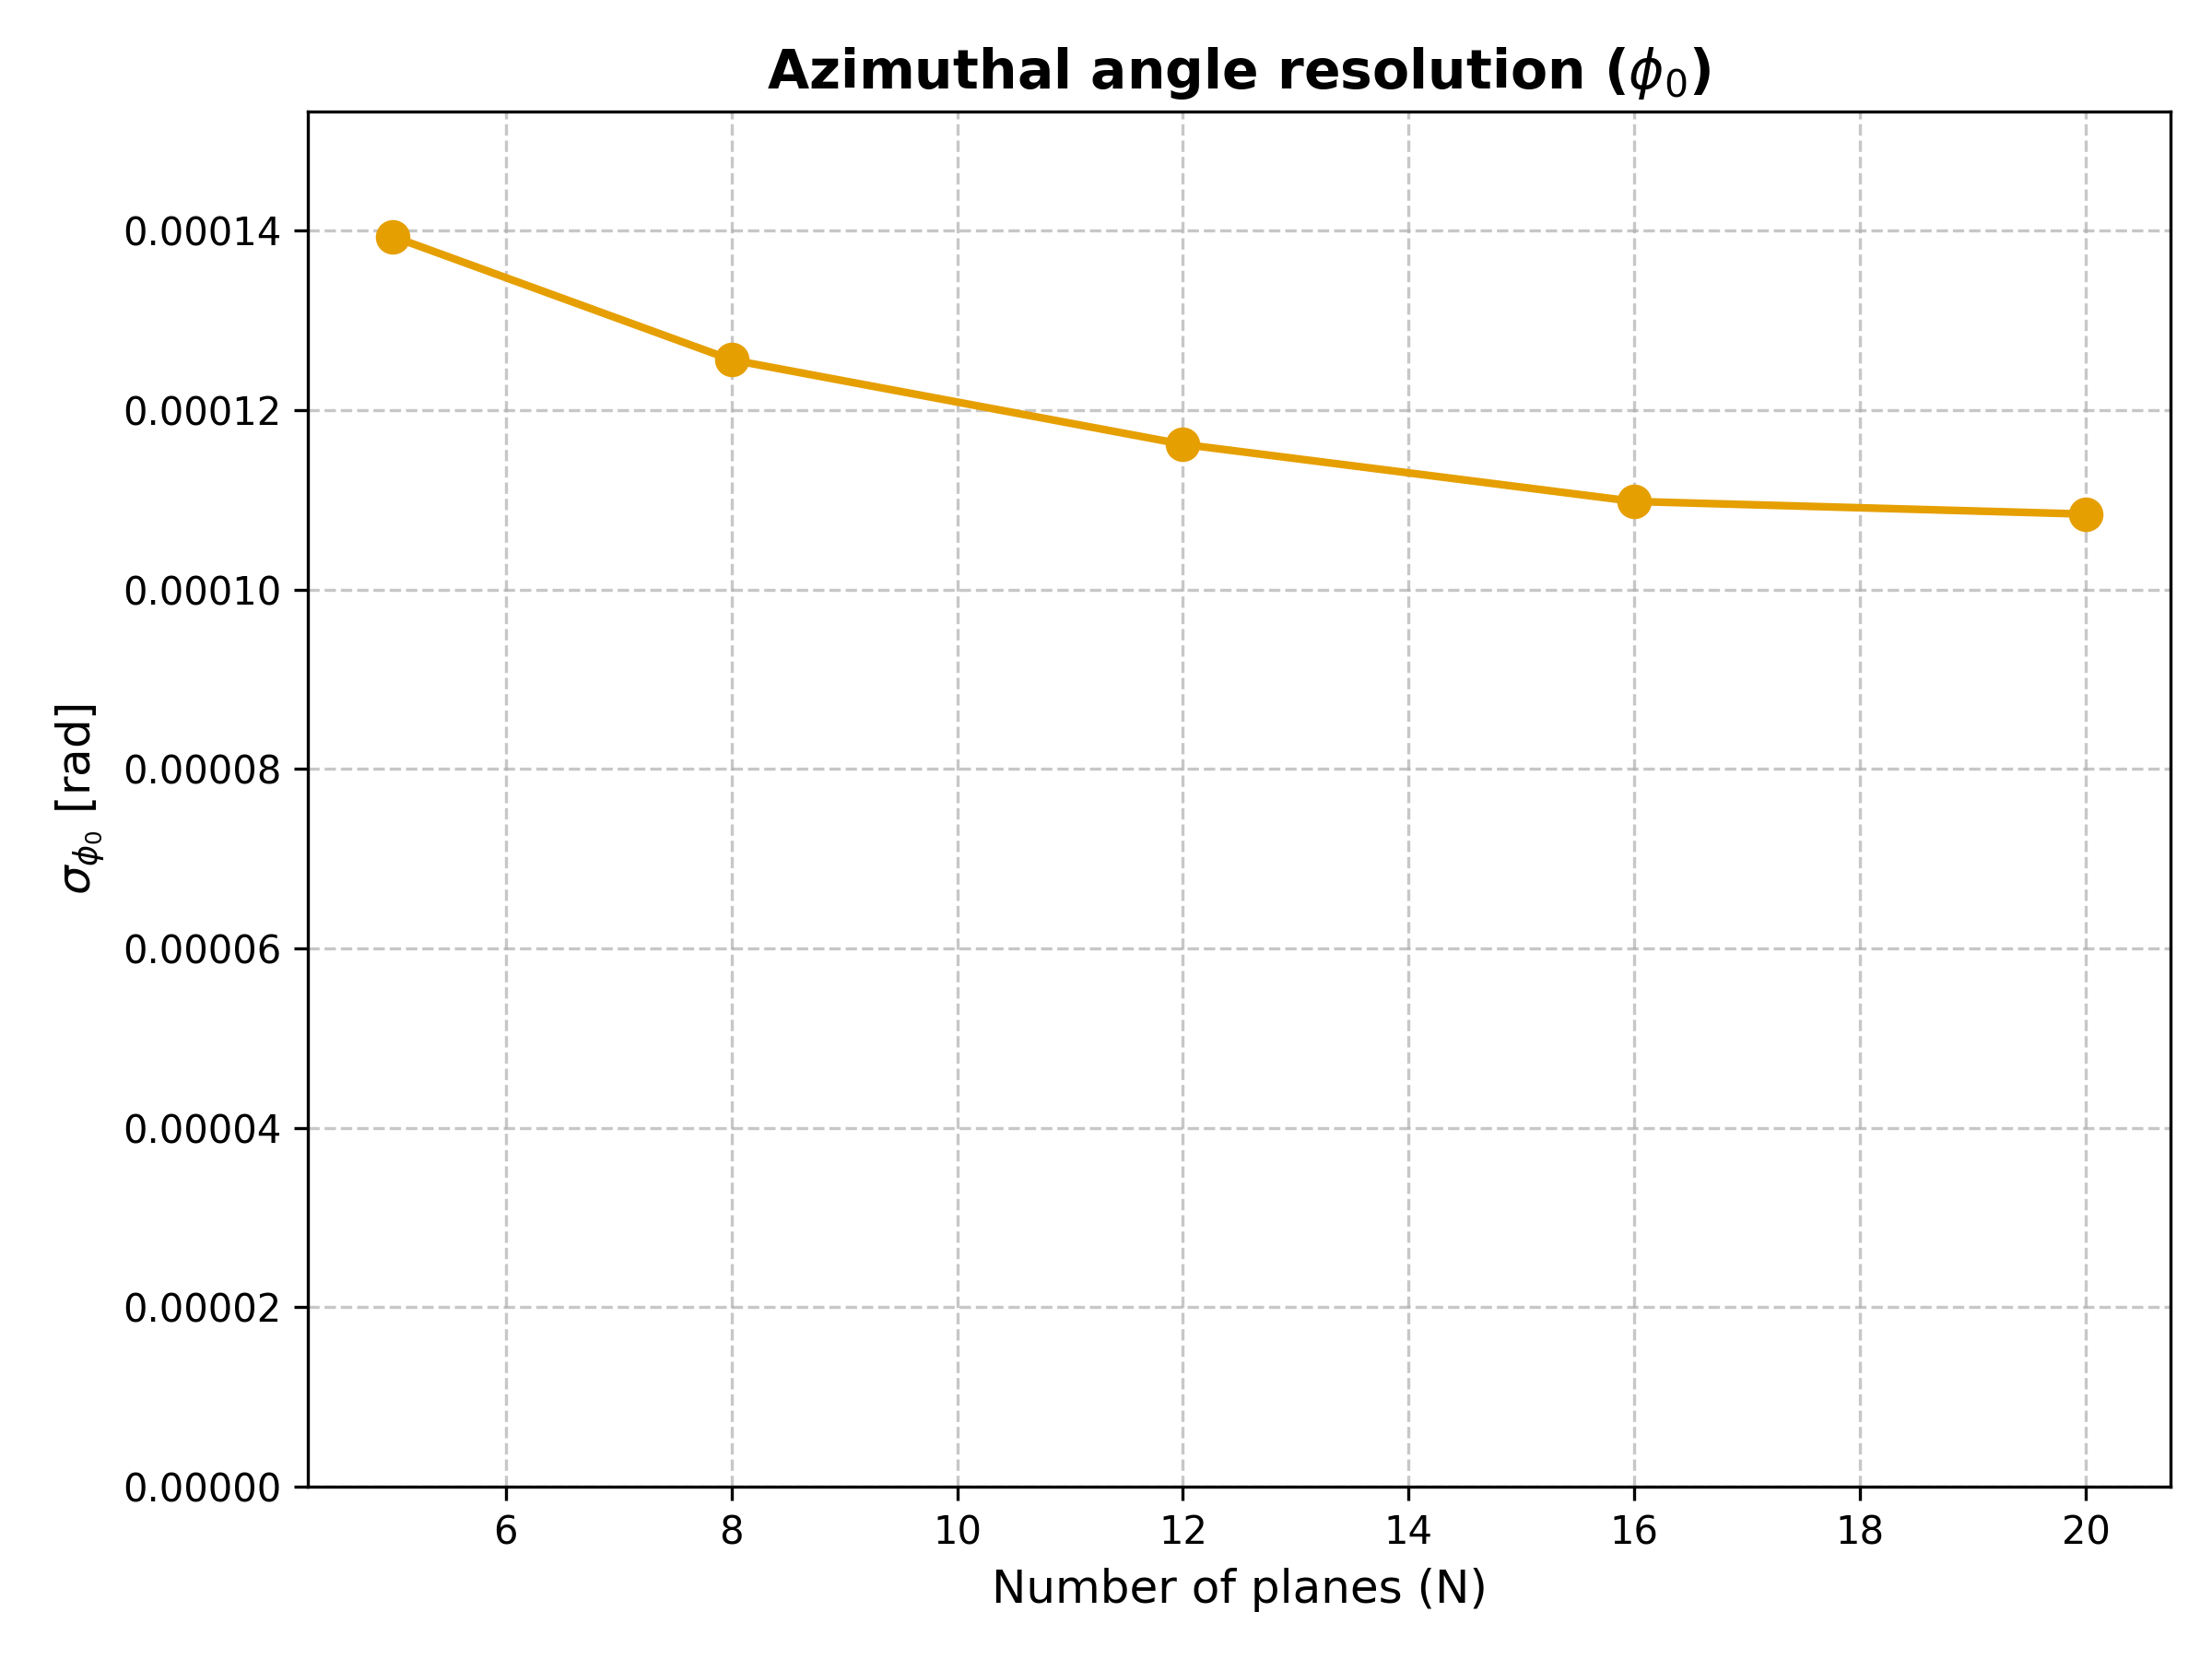
\includegraphics[width=0.85\textwidth]{Immagini/trend_phi0.png}
        \end{column}
    \end{columns}
\end{frame}

\begin{frame}{Exercise 3.2: Global parameters resolution ($\kappa$ \& $\sigma_p/p$)}
    \begin{itemize}
        \item \textbf{Curvature ($\kappa$):} Initially improves statistically, but begins to degrade at $N\sim20$ planes as the added material introduces significant multiple scattering.
        \item \textbf{Momentum ($\sigma_p/p$):} Mirrors the curvature, clearly showing the physical trade-off between higher spatial sampling density and cumulative scattering noise.
    \end{itemize}
    
    
    \begin{columns}
        \begin{column}{0.5\textwidth}
            \centering
            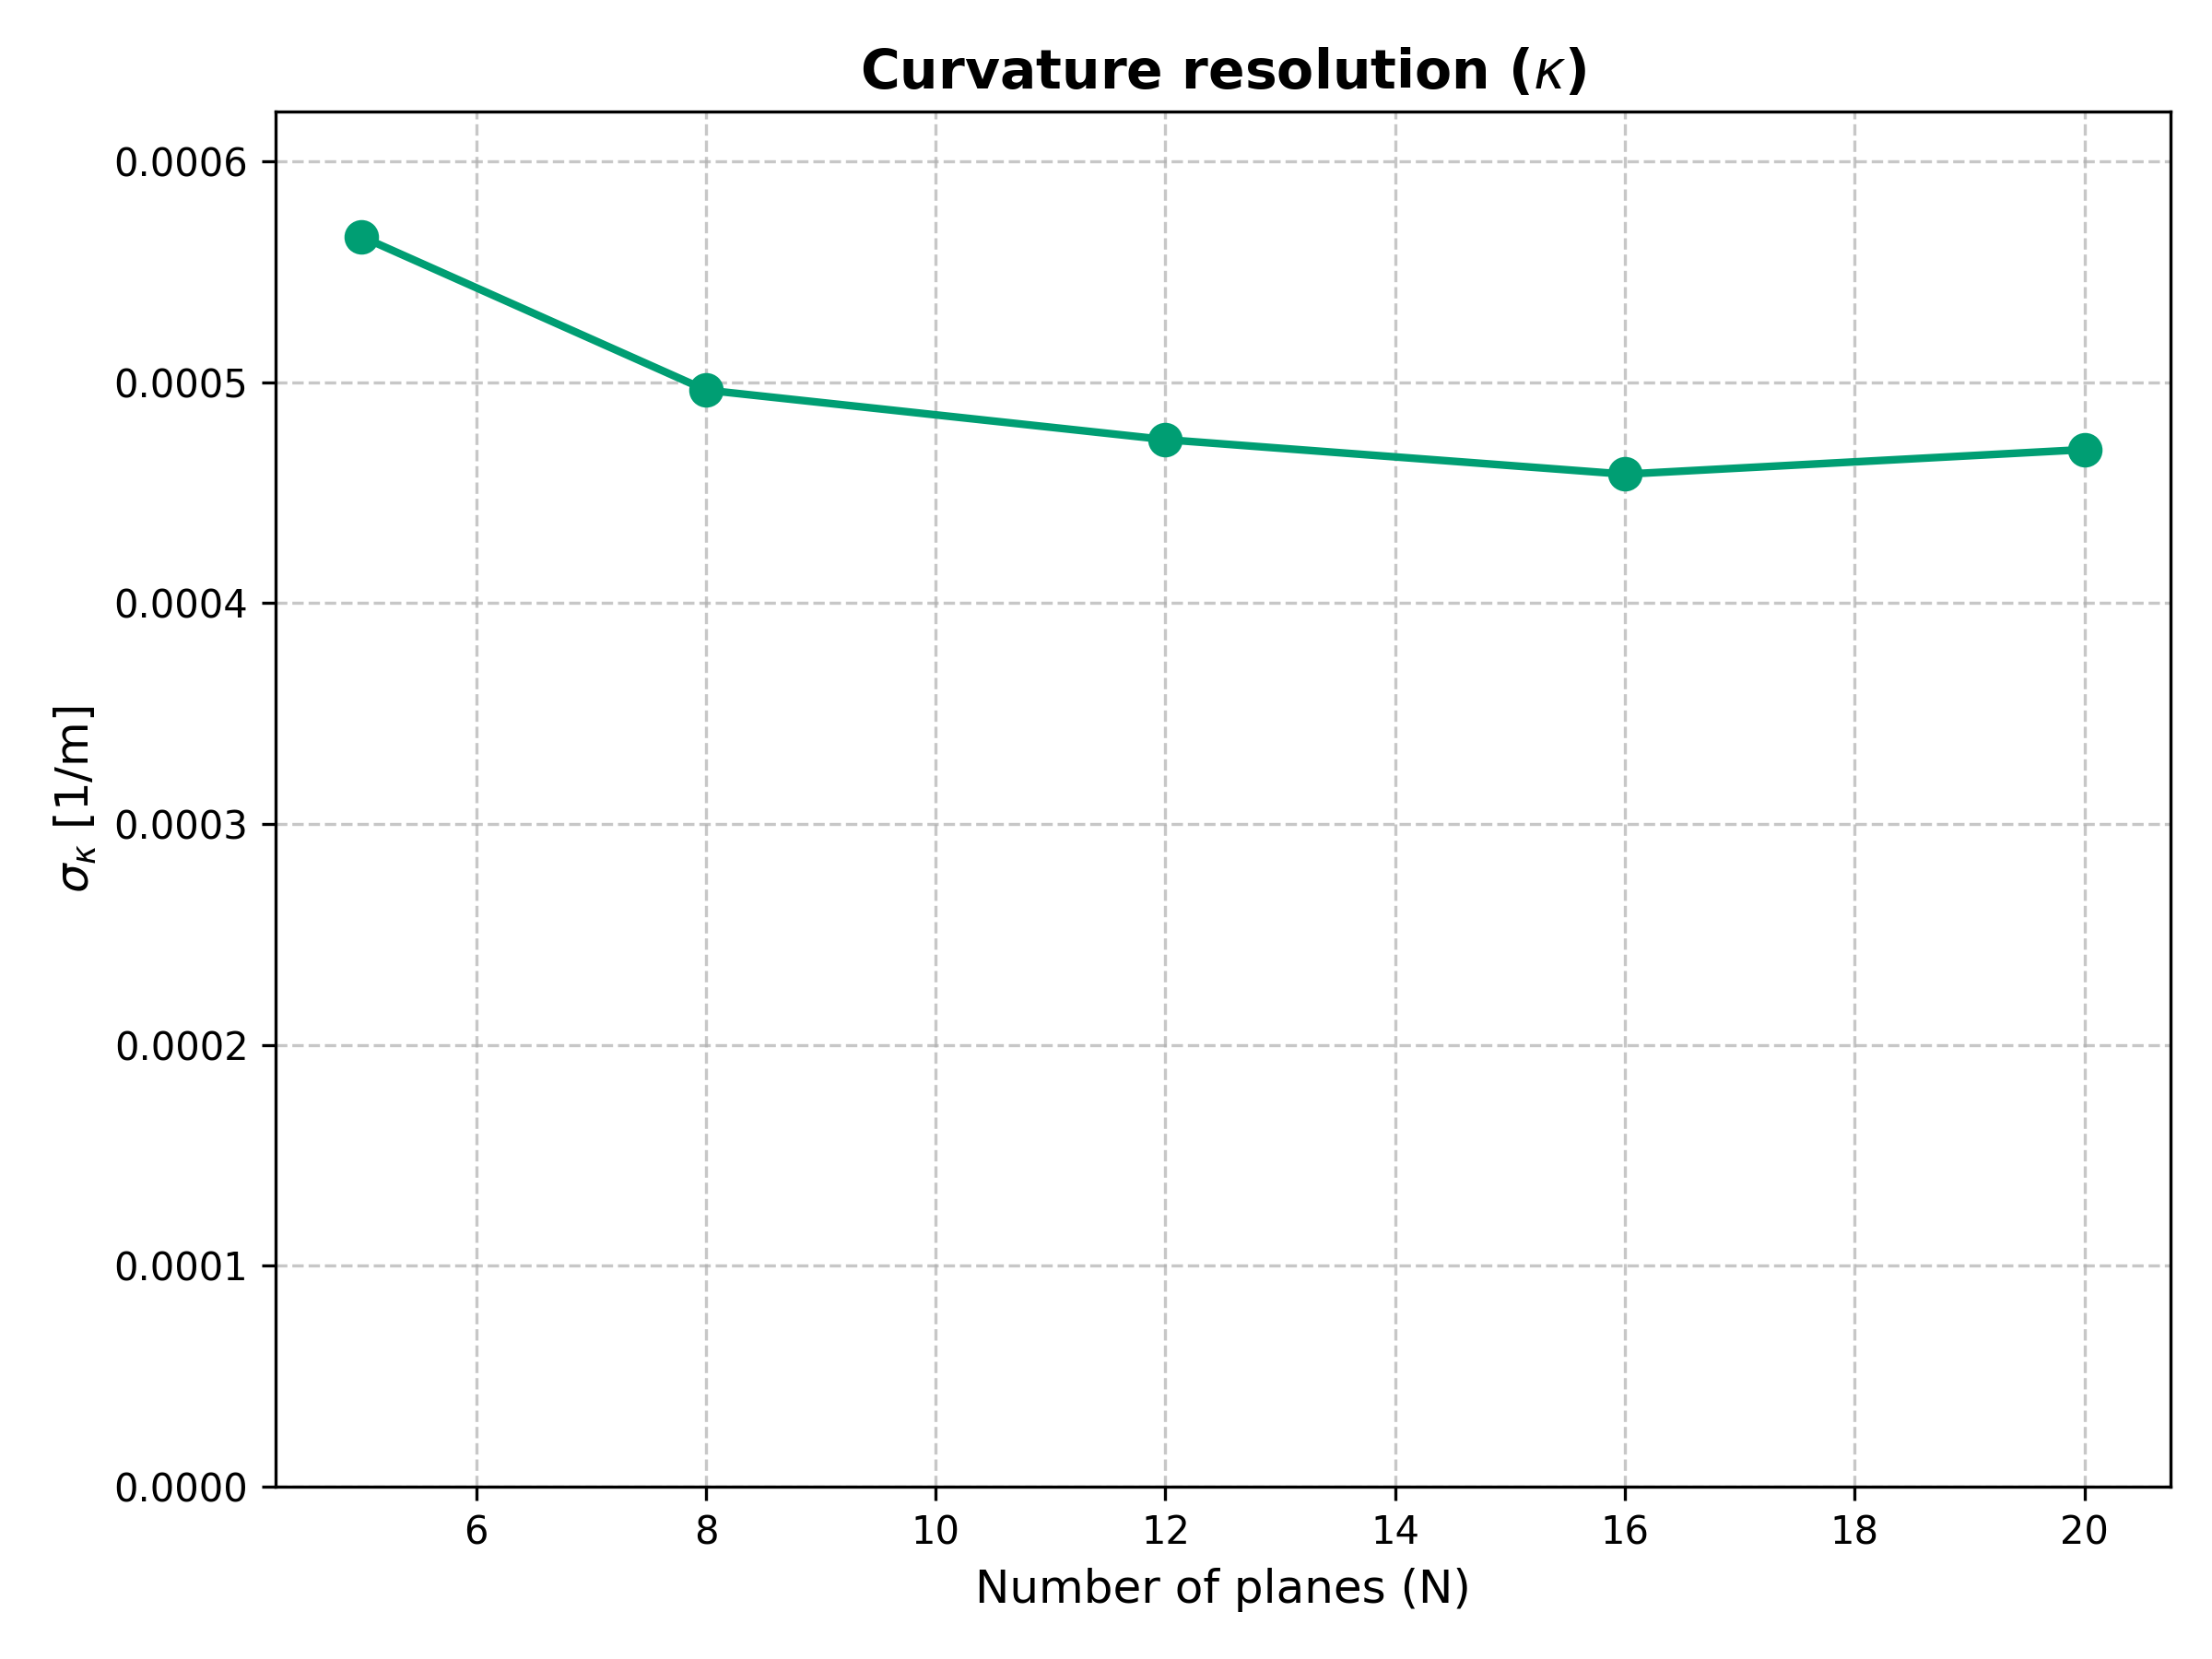
\includegraphics[width=0.85\textwidth]{Immagini/trend_kappa.png}
        \end{column}
        \begin{column}{0.5\textwidth}
            \centering
            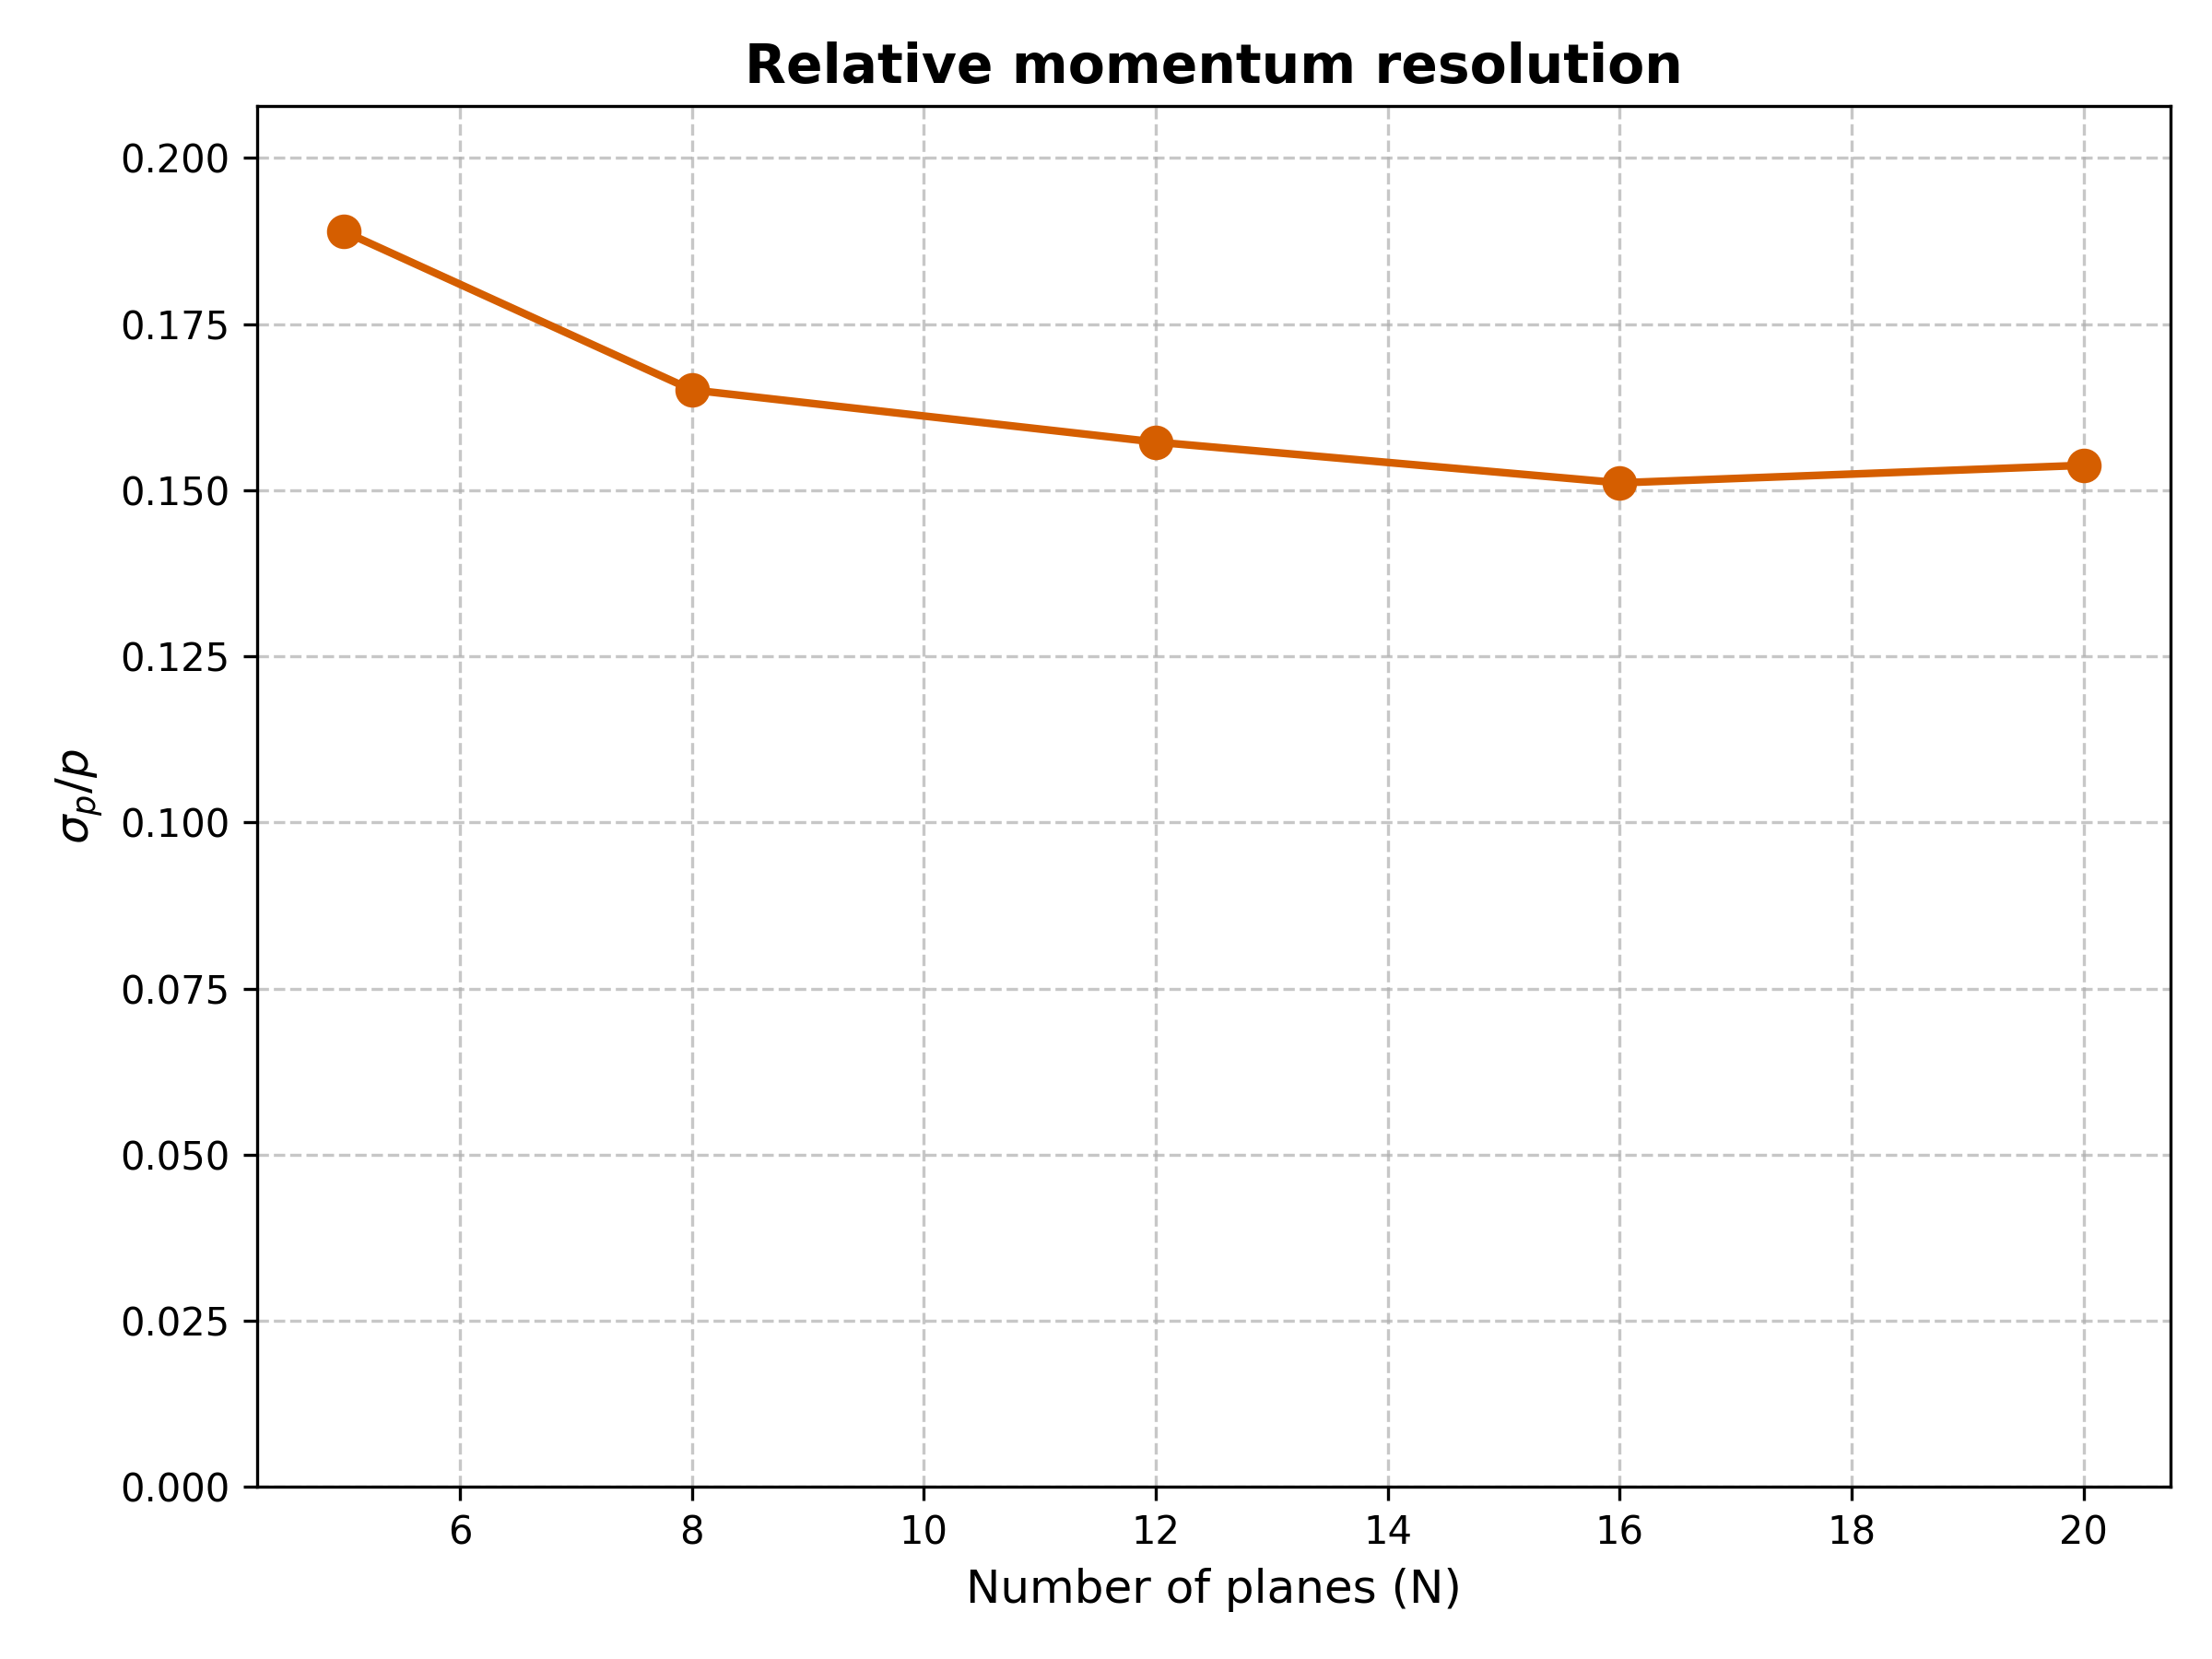
\includegraphics[width=0.85\textwidth]{Immagini/trend_momentum.png}
        \end{column}
    \end{columns}
\end{frame}


\begin{frame}{Exercise 3.3: Increasing the lever arm}
    \begin{itemize}
        \item Doubling the spacing between the 5 planes doubles the total lenght $L$ (from 40 cm to 80 cm), keeping the material constant.
        \item Geometric limits predict $\sigma_\kappa \propto 1/L^2$. 
        Conversely, $\sigma_{d_0}$ with the standard spacing already satisfies $n \gg 1$ implies only a marginal gain with larger $L$.
    \end{itemize}
        
    \begin{table}[]
        \centering
        \renewcommand{\arraystretch}{1.3}
        \resizebox{\textwidth}{!}{
        \begin{tabular}{l|c|c|c}
            \textbf{Resolution} & \textbf{Standard Spacing} & \textbf{Doubled Spacing} & \textbf{Improvement Ratio} \\
            \hline
            $\sigma_{d_0}$ [mm]      & $1.47 \times 10^{-2}$ & $1.17 \times 10^{-2}$ & \textbf{$\sim 1.26$}  \\
            $\sigma_{\phi_0}$ [rad]  & $1.39 \times 10^{-4}$ & $6.49 \times 10^{-5}$ & \textbf{$\sim 2.14$}  \\
            $\sigma_\kappa$ [$m^{-1}$] & $5.66 \times 10^{-4}$ & $1.39 \times 10^{-4}$ & \textbf{$\sim 4.07$} (Expected $\approx 4$) \\
            $\sigma_p/p$             & $1.89 \times 10^{-1}$ & $4.66 \times 10^{-2}$ & \textbf{$\sim 4.065$} (Expected $\approx 4$) \\
        \end{tabular}
        }
    \end{table}
    
\end{frame}


% --- FRAME 1 ---
\begin{frame}{Exercise 4: Kinematics of $J/\psi \rightarrow \mu^+\mu^-$ decay}
    \begin{itemize}
        \item \textbf{Muon kinematics:} Assuming a symmetric decay, the muon momentum $p_\mu$ and opening angle $\phi$ are derived from the invariant mass:
        $$ p_\mu = \sqrt{(E_{J/\psi}/2)^2 - m_\mu^2} \quad \text{and} \quad \cos\phi = 1 - \frac{m_{J/\psi}^2}{2p_\mu^2} $$
        \item \textbf{Boost and $B_s^0$ decay:} The Lorentz factor is $\gamma\beta = p_{J/\psi} / m_{J/\psi}$, so the expected decay length is $L_B = \gamma\beta c\tau_B$, with intrinsic $c\tau_B = 450~\mu$m.
        \item \textbf{Invariant mass:} In the ultrarelativistic approximation, $E_\mu \simeq p_\mu c$ and, for a symmetric decay, $M_{\mu\mu} \simeq 2p_\mu\sin(\phi/2)$. Both cases give $M_{\mu\mu} \simeq 3.09\,\mathrm{GeV}/c^2$, consistent with the $J/\psi$ mass.
    \end{itemize}
\end{frame}

% --- FRAME 2 ---
\begin{frame}{Exercise 4: Error propagation model}
    \begin{itemize}
        \item \textbf{Vertex resolution ($\sigma_{vertex}$):} Error propagation from the geometric intersection of the two outgoing tracks in a symmetric decay:
    $$ \sigma_{vertex} = \frac{\sigma_{d_0}}{\sqrt{2}\tan(\varphi/2)} $$
        \item \textbf{Invariant mass relative errors ($\sigma_M/M$):} Propagating relative errors for uncorrelated variables $p$ and $\phi$:
        $$ \frac{\sigma_M}{M} = \sqrt{\left(\frac{\sigma_p}{p}\right)^2 + \left(\frac{\sigma_\phi}{2 \tan\left(\frac{\phi}{2}\right)}\right)^2} $$
    \end{itemize}
\end{frame}

% --- FRAME 3 --
\begin{frame}{Exercise 4: Simulation results}
    \begin{columns}[T]
        \begin{column}{0.49\textwidth}
            \begin{table}[]
                \centering
                \renewcommand{\arraystretch}{1.25}
                \caption{Calculated kinematic balues}
                \vspace{\baselineskip}
                \begin{tabular}{lcc}
                    \hline
                    \textbf{Parameter} & \textbf{Case A} & \textbf{Case B} \\ \hline
                    $p_\mu \, [\text{GeV}/c]$ & 1.624 & 5.233 \\
                    $\phi$ & 145.0$^\circ$ & 34.4$^\circ$ \\
                    $L_B\, [\text{mm}]$ & 0.145  & 1.453  \\ \hline
                \end{tabular}
            \end{table}
        \end{column}
        \begin{column}{0.49\textwidth}
            \begin{table}[]
                \centering
                \renewcommand{\arraystretch}{1.25}
                \caption{Extracted resolutions and derived errors}
                \begin{tabular}{lcc}
                    \hline
                    \textbf{Uncertainty} & \textbf{Case A} & \textbf{Case B} \\ \hline
                    $\sigma_{d_0} \, [\text{mm}]$ & 0.046  & 0.021  \\
                    $\sigma_\kappa\, [\text{m}^{-1}]$ & 0.005  & 0.002  \\
                    $\sigma_{vertex}$\, [\text{mm}] & 0.01  & 0.04  \\
                    $\sigma_M/M\, [\%]$ & 2.75  & 3.39  \\ \hline
                \end{tabular}
            \end{table}
        \end{column}
    \end{columns}
\end{frame}

% --- FRAME 4 ---
\begin{frame}{Exercise 4: Discussion and conclusions}
    \begin{itemize}
        \item In both simulated regimes, the vertex resolution is strictly smaller than the expected flight length ($\sigma_{vertex} < L_B$). This confirms the detector's capability to separate secondary $J/\psi$ decays from prompt primary vertices.
        \item The angular contribution to the invariant mass variance ($\sim 10^{-7}$) is completely negligible compared to the momentum measurement error ($\sim 10^{-3}$).
        \item The resulting mass resolution ($\sim 100$ MeV/c$^2$) completely masks the intrinsic $J/\psi$ natural width of 93 keV. 
    \end{itemize}
\end{frame}


% ==================///==================///==================///
% ==================/// END PRESENTATION
% ==================///==================///==================///

\backmatter
\appendix
\section*{BACKUP}
\begin{frame}[noframenumbering]
    \begin{center}
        \Huge \textbf{BACKUP}
    \end{center}
\end{frame}

\begin{frame}[noframenumbering]{Invariant mass resolution}
    
    \footnotesize
    
    For a symmetric 2-body decay (e.g., $J/\psi \to \mu^+\mu^-$ where $p_1 = p_2 \equiv p_\mu$), the invariant mass simplifies to:
    \begin{equation*}
        M_{\mu\mu} \approx 2 p_\mu \sin\left(\frac{\phi}{2}\right)
    \end{equation*}
    
    
    Applying relative error propagation yields a compact formula driven by two main terms:
    \begin{equation*}
        \frac{\sigma_{M_{\mu\mu}}}{M_{\mu\mu}} = \sqrt{ \left(\frac{\sigma_{p_\mu}}{p_\mu}\right)^2 + \left(\frac{\sigma_\phi}{2\tan(\phi/2)}\right)^2 }
    \end{equation*}
    
    
    \begin{itemize}
        \item \textbf{Momentum term:} The relative momentum resolution is directly determined by the curvature ($\kappa$) resolution of the tracker:
        \begin{equation*}
            \frac{\sigma_{p_\mu}}{p_\mu} = \frac{\sigma_\kappa}{\kappa}
        \end{equation*}
        
        \item \textbf{Angular term ($\phi = \phi_1 - \phi_2$):} Assuming independent and identical angular measurement errors for both tracks ($\sigma_{\phi_1} = \sigma_{\phi_2} \equiv \sigma_{\phi_0}$):
        \begin{equation*}
            \sigma_\phi = \sqrt{\sigma_{\phi_1}^2 + \sigma_{\phi_2}^2} = \sqrt{2}\sigma_{\phi_0}
        \end{equation*}
    \end{itemize}

\end{frame}

\begin{frame}[noframenumbering]{Vertex resolution derivation}
    
    \footnotesize
    
    \begin{columns}[T]
        % Colonna di sinistra: Geometria
        \begin{column}{0.48\textwidth}
            Symmetric decay along the $x$-axis with opening angle $\varphi$. Linear track approximation near the origin:
            \begin{align*}
                y_1 &= \tan(\varphi/2) x + d_1 \\
                y_2 &= -\tan(\varphi/2) x + d_2
            \end{align*}
            
            \vspace{0.4cm}
            
            Equating the trajectories ($y_1 = y_2$) to find the intersection point along the flight direction:
            \begin{equation*}
                x_v = \frac{d_2 - d_1}{2\tan(\varphi/2)}
            \end{equation*}
        \end{column}
        
        % Colonna di destra: Propagazione errori
        \begin{column}{0.48\textwidth}
            Assuming negligible angular uncertainty and independent, identical impact parameter errors ($\sigma_{d_1} = \sigma_{d_2} \equiv \sigma_{d_0}$):
            \begin{equation*}
                \sigma_{x_v}^2 = \left(\frac{\partial x_v}{\partial d_1}\right)^2 \sigma_{d_0}^2 + \left(\frac{\partial x_v}{\partial d_2}\right)^2 \sigma_{d_0}^2
            \end{equation*}
            
            \vspace{0.2cm}
            
            Evaluating the partial derivatives directly yields the longitudinal resolution:
            \begin{equation*}
                \sigma_{x_v} = \sqrt{ \frac{\sigma_{d_0}^2}{4\tan^2(\varphi/2)} + \frac{\sigma_{d_0}^2}{4\tan^2(\varphi/2)} }
            \end{equation*}
            
            \vspace{-0.2cm} % Compressione per far risaltare il risultato finale
            \begin{equation*}
                \sigma_{x_v} = \frac{\sigma_{d_0}}{\sqrt{2}\tan(\varphi/2)}
            \end{equation*}
        \end{column}
    \end{columns}

\end{frame}



\end{document}